\documentclass[journal]{IEEEtran}
\usepackage{graphicx}
\usepackage{amsmath}
\usepackage{booktabs}
\usepackage{url}
\usepackage[hidelinks]{hyperref}
\graphicspath{{figures/}}

\begin{document}

\title{Launch-Blind Product Viability Estimation from Specifications via LLM Aspect Bridging}

\author{Raj~Jagtap%
\thanks{R. Jagtap is an undergraduate student of Computer Science and Engineering. This work was completed as a final-year capstone project, 2026.}}

\maketitle

\begin{abstract}
Product teams commit manufacturing and development budgets before a single consumer has used what they are building, yet the methods that predict product success all depend on post-launch signals such as reviews or sales. This paper describes a pipeline that works before launch. A large language model extracts aspect-level sentiment from more than 74{,}000 real consumer reviews under a null-forcing prompt; gradient-boosted models then learn which aspect profiles succeed within each category; and a bridging layer, prompted to reason skeptically and grounded in category statistics, estimates the aspect profile that an unseen product would earn from its specifications alone. We evaluated this on a pre-registered holdout of 59 real products, sampled before any tuning with the pipeline frozen. Specs-only predictions rank those products against their actual market outcomes at Spearman $\rho = 0.317$ (95\% CI $[0.06, 0.54]$) and separate eventual bottom-quintile from top-quintile products at AUC $= 0.743$. The signal is almost orthogonal to a price-percentile baseline ($r = 0.135$), so it carries information beyond price position. Two negative results are reported with the same care as the positive ones. The same method fails for mobile applications across five outcome definitions (best $R^2 = 0.231$), the pattern one expects when a market rewards distribution over quality. Injecting Reddit-derived consumer priorities raises performance by $\rho$ $+0.049$, but the bootstrap interval includes zero, so we label that lift exploratory rather than confirmed. Throughout, the system reports its own measured limits through per-aspect trust tiers, grounding flags, and abstention, which we argue any honest pre-production tool has to do.
\end{abstract}

\begin{IEEEkeywords}
Product success prediction, aspect-based sentiment analysis, large language models, gradient boosting, pre-launch analytics, electronic word of mouth.
\end{IEEEkeywords}

\section{Introduction}
\IEEEPARstart{L}{arge} enterprises evaluate prospective products with market-research departments, paid consumer panels, and proprietary analytics. A small business or independent maker has none of that. The decision to manufacture a wireless headphone or publish a mobile application is usually made on intuition, a scan of competitors, and hope. The cost of being wrong is not abstract: an unsold inventory run or a failed development cycle can end a small firm. It falls on consumers too, who pay for products that break, disappoint, or were never matched to what they needed in the first place. This work sets out to narrow that gap. We want to give businesses without expensive market-intelligence tooling an affordable, evidence-based estimate of whether a product design is likely to satisfy its market \emph{before} money is committed to building it, so that the products that do get built are more likely to be worth what their users pay for them.

The obstacle here is structural, not incidental. Decades of work relate online reviews and electronic word of mouth (e-WOM) to sales and market outcomes \cite{chevalier2006wom,dellarocas2003digitization,chintagunta2010effects,luca2016reviews}, and modern sentiment pipelines pull remarkably fine-grained signals out of review text \cite{zhang2022survey,wang2025multifeature,shan2025bilingual}. Every one of these methods consumes \emph{post-launch} data. At the moment the decision matters most, before production, there are no reviews, no ratings, and no sales. All that exists is the product's specification and whatever the category it will enter has taught us so far.

This paper asks whether that is enough. The central idea is \emph{aspect bridging}. We first learn, from more than 74{,}000 real reviews, how consumers in each category score products along interpretable quality aspects (build quality, ease of use, value for money, and so on), and how those profiles relate to eventual market success. We then ask a large language model, prompted as a skeptical market analyst and grounded in per-category statistics, to estimate the aspect profile that an \emph{unseen} product would earn from its specification alone. That estimated profile goes into the trained success model, which returns a launch-blind viability estimate along with per-aspect explanations, measured trust tiers, and an explicit abstention when the specification offers too little to go on.

A system meant to inform real financial decisions has to be validated with matching rigor, so our primary contribution is methodological. The evaluation is launch-blind: each real product is re-judged from only what was knowable on its launch day, and the prediction is then compared against the market outcome it actually earned. After all the design iterations on a development set, we \emph{pre-registered} a confirmatory holdout with a disjoint sample, a frozen pipeline, and pre-specified metrics, following the preregistration movement in empirical science \cite{nosek2018preregistration}. The contributions are:

\begin{itemize}
\item \textbf{C1.} A null-forcing aspect-extraction scheme over 74{,}000+ reviews in which an LLM may score an aspect only with verbatim textual evidence, never by inference, with typed validation and a crash-safe multi-provider pipeline (Section~\ref{sec:method}).
\item \textbf{C2.} The bridging layer: a skeptic-prompted, category-grounded LLM estimator of aspect profiles from specifications, with absence penalties, grounding flags, and anchor discipline (Section~\ref{sec:method}).
\item \textbf{C3.} A retrospective launch-blind validation harness and a pre-registered confirmatory holdout confirming a real, price-complementary signal: $\rho = 0.317$, CI $[0.06,0.54]$, AUC $=0.743$ (Section~\ref{sec:validation}).
\item \textbf{C4.} An honest map of scope: which aspects specifications can predict and which they cannot, and a five-target negative result showing the method fails for mobile applications (Section~\ref{sec:negative}).
\item \textbf{C5.} A measured, paired A/B evaluation of community-derived consumer priorities as bridging context (Section~\ref{sec:reddit}), and a deployed decision-support application whose interface surfaces the system's own measured limitations (Section~\ref{sec:system}).
\end{itemize}

\section{Related Work}
\label{sec:related}

\subsection{Reviews, e-WOM, and Market Outcomes}
That online opinion moves markets is well established. Chevalier and Mayzlin showed that review valence shifts book sales across retailers \cite{chevalier2006wom}; Dellarocas framed digitized word of mouth as a new economic feedback mechanism \cite{dellarocas2003digitization}; Chintagunta et al.\ tied user reviews to box-office trajectories \cite{chintagunta2010effects}; and Luca measured the revenue effects of Yelp ratings \cite{luca2016reviews}. Closer to our feature level, Archak et al.\ showed that \emph{aspect-level} review content carries pricing power beyond the star rating \cite{archak2011deriving}, Ghose and Ipeirotis linked review-text characteristics to economic impact \cite{ghose2011estimating}, and Mudambi and Schuff studied what makes a review informative \cite{mudambi2010helpful}. Social-media signals have been used the same way to forecast outcomes \cite{asur2010predicting}. All of this work operates after launch. The closest antecedent to our goal is the pre-launch prediction of Narayanan et al., which forecasts reception from pre-release chatter about announced products \cite{narayanan2020prelaunch}. Our setting is strictly harder, because we assume no product-specific chatter exists at all, only the specification and the history of the category.

Review streams are also adversarial. Opinion spam has been studied since Jindal and Liu \cite{jindal2008opinion}, deceptive reviews can be manufactured convincingly \cite{ott2011deceptive}, and there is a clear economic incentive to manipulate them \cite{mayzlin2014promotional}. The corpus-level fraud filter in Section~\ref{sec:data} follows this line of work.

\subsection{Aspect-Based Sentiment Analysis}
Aspect-based sentiment analysis (ABSA) began with frequency- and lexicon-based aspect mining \cite{hu2004mining,liu2012sentiment}, was standardized by the SemEval-2014 benchmark \cite{pontiki2014semeval}, and has since been dominated by neural approaches, surveyed in \cite{zhang2022survey}. Recent systems keep refining the extraction machinery, with multi-feature fusion graph attention networks \cite{wang2025multifeature}, curriculum-learning hybrids \cite{lange2025curriculum}, transformer pipelines for bilingual e-commerce satisfaction \cite{shan2025bilingual}, and multi-source sentiment fusion \cite{sesr2025multisource}. What sets our work apart is the purpose, not the machinery. We treat ABSA as a \emph{measurement instrument} that turns unstructured reviews into a per-product aspect profile, which then becomes the substrate for supervised learning, and we impose a null-forcing, evidence-quoting discipline aimed at downstream trustworthiness rather than benchmark accuracy.

\subsection{LLMs as Extractors and Estimators}
Transformer language models \cite{vaswani2017attention,devlin2019bert}, scaled into instruction-following generalists \cite{brown2020gpt3,ouyang2022instruct,openai2023gpt4,gemini2023,touvron2023llama}, now annotate text about as well as human crowds \cite{gilardi2023chatgpt} and show up more and more as zero-shot components in e-commerce pipelines: product classification \cite{roumeliotis2025llms}, description generation from reviews \cite{gutierrez2025zeroshot}, and numeric value prediction in industrial systems \cite{hidayat2025custody}. Reasoning-eliciting prompting \cite{wei2022chain} and the broader foundation-model programme \cite{bommasani2021foundation} frame LLMs as general-purpose estimators. Our bridging layer sits in this line but adds two disciplines that are rarely evaluated together: skepticism about adversarial input, since marketing copy is written to sound optimistic for flops and hits alike, and \emph{launch-blind outcome validation}, which checks the LLM's estimates against the market reality that followed.

\subsection{Gradient Boosting for Tabular Prediction}
For tabular product features, gradient-boosted trees \cite{friedman2001greedy,chen2016xgboost,ke2017lightgbm} are still the strong default, ahead of both classic ensembles \cite{breiman2001random} and neural alternatives, and they appear across e-commerce supply chains \cite{sayyad2024catboost}, sentiment-augmented financial forecasting \cite{zhen2025stock,shang2025bitcoin}, and multi-criteria recommendation \cite{rakee2025temul}. We use XGBoost for its native handling of missing values (an unmentioned aspect stays missing rather than being imputed) and SHAP attributions \cite{lundberg2017shap} to turn predictions into design-lever explanations. The data infrastructure builds on the Amazon reviews corpora \cite{he2016ups,hou2024amazon} and the archived Reddit ecosystem \cite{baumgartner2020pushshift}, and we quantify uncertainty with the bootstrap \cite{efron1979bootstrap}. One more connection is worth naming: our insistence that the interface display the model's limits echoes recent management-literature arguments that AI-assisted decisions need calibrated human autonomy \cite{cristofaro2026dancing}.

\section{Data}
\label{sec:data}
The corpus spans two market types. Physical products come from the Amazon Reviews 2023 dataset \cite{hou2024amazon} across six categories (wireless headphones, Bluetooth speakers, smartphones, smartwatches, power banks, and kitchen appliances). Mobile applications come from Google Play across four (finance, health \& fitness, productivity, and education). We cleaned reviews to English text of 10--400 words, kept only products with at least five reviews, and normalized timestamps; all ratings lie in $[1,5]$. After cleaning, the corpus holds 1{,}051 products (732 physical, 319 app), and the extraction stage processed over 74{,}000 reviews.

Review streams can be gamed \cite{jindal2008opinion,mayzlin2014promotional}, so we ran a fraud filter before building labels. A product was flagged if more than 40\% of its sampled reviews fell inside a single 14-day window, if its rating distribution was extreme-J-shaped, or if more than 30\% of its reviews were near-duplicates (Jaccard $> 0.7$ on word sets). This excluded 71 products from training.

The regression target is a within-category composite. For physical products, $\text{success} = 100\,(0.40\,\text{volume} + 0.35\,\text{rating} + 0.25\,\text{velocity})$, with each component min--max normalized inside its category and $\log(1+x)$ applied to the heavy-tailed counts. Apps add install counts and a retention proxy (rating count divided by install count). Normalizing within category matters: 500 reviews means one thing for a kitchen appliance and something quite different for a smartphone.

\textbf{Survivorship disclosure.} The five-review floor means that products which launched and drew no attention at all never enter the corpus. Every claim in this paper is therefore about ranking among products that did reach the market's attention. When we say ``flop'' we mean the bottom success quintile of these survivors, not a product nobody bought. Section~\ref{sec:limitations} works through what this costs us.

For the exploratory study of Section~\ref{sec:reddit} we also collected 1{,}089 buying-intent Reddit comments across all ten categories through the Arctic Shift archive of Reddit \cite{baumgartner2020pushshift}, taking threads with purchase-decision titles and comments scoring $\geq 5$, of 10--400 words, with near-duplicates removed. Coverage is uneven, and we disclose it: 237 comments for health \& fitness apps at one end, 18 for smartphones at the other. We make no per-category claims from this source.

\section{Method}
\label{sec:method}

\subsection{Aspect Extraction}
Each review is decomposed into aspect-level sentiment against a frozen schema of six aspects shared across market types (value for money, utility, ease of use, reliability, design appeal, after-sales), three physical-only aspects (build quality, durability, repairability), and five app-only aspects (performance, stability, ad experience, update support, privacy/trust). The extraction prompt is deliberately \emph{null-forcing}. An aspect may be scored (0--10) only if the review explicitly discusses it; every non-null score must carry a verbatim evidence phrase copied from the review; and the reviewer's star rating is given as context but is forbidden as a source of scores. A review that praises only sound quality returns nulls for durability, because silence is data we will not fabricate. Outputs are validated against typed schemas. An invalid response is retried once with the error appended, then failed over to the next provider, and after a third failure the review is logged and skipped, so no single bad response can stall a multi-day batch. Extraction ran over more than 74{,}000 reviews on a multi-provider pool (Gemini Flash, Groq Llama-3.3-70B, and a local fallback) with per-key rate tracking, append-only crash-safe logging, and resume support. Before the full batch, a 30-review hand-validation gate checked that unmentioned aspects came back null and that every evidence phrase actually appeared in its review.

\subsection{Success Models and Algorithm Selection}
\label{sec:models}
Product-level features aggregate the extraction stream into a per-aspect mean score and a mention rate. An aspect that is never mentioned stays missing rather than imputed, which XGBoost \cite{chen2016xgboost} handles natively. To these we add metadata: price, average rating, log rating count, review velocity, and category. We train gradient-boosted regressors (600 estimators, depth 5, learning rate 0.05, seed 42) under 5-fold cross-validation, and we report two variants that carry very different epistemic weight. The \emph{full} model reaches CV $R^2 = 0.893$ on physical products, but 35\% of its target is the average rating that it also receives as a feature. We disclose this leakage and read the number as an upper bound on fit, not as evidence of insight. The \emph{aspects-only} variant, with metadata stripped and only LLM features left, reaches $R^2 = 0.567$ on physical products, and it is the variant behind every claim in this paper. The same variant scores $R^2 = 0.101$ for apps, the negative finding we examine in Section~\ref{sec:negative}.

\textbf{Why XGBoost.} We did not assume the learning algorithm. Six algorithms were benchmarked on the identical aspects-only feature matrix under the same 5-fold CV (seed 42, $n = 732$ physical products), and Table~\ref{tab:algo} with Fig.~\ref{fig:algometrics} report every metric. XGBoost has the highest $R^2$ (0.564), the lowest RMSE (11.4), and the highest AUC-ROC for top-vs-bottom quintile discrimination (0.983), and it trains in 0.29\,s, which is 2.5$\times$ faster than Random Forest and 8$\times$ faster than sklearn Gradient Boosting. The runner-up, sklearn Gradient Boosting ($R^2 = 0.549$), matches XGBoost on AUC but takes 7$\times$ longer, since it lacks histogram-based splitting \cite{ke2017lightgbm}. Random Forest \cite{breiman2001random} ($R^2 = 0.532$) and the MLP ($R^2 = 0.490$) fall behind, and the gap down to SVR \cite{cortes1995svm} ($R^2 = 0.421$) and Ridge Regression \cite{hoerl1970ridge} ($R^2 = 0.368$) confirms that the nonlinear interactions matter. This lines up with recent large-scale benchmarks in which tree ensembles beat deep learning on typical tabular data \cite{grinsztajn2022tree,shwartzziv2022tabular}.

Accuracy aside, three properties of this problem favor XGBoost. The first is native missing-value handling. Aspect scores are structurally missing whenever a review does not mention an aspect, and XGBoost learns a split direction for missing entries without imputation \cite{chen2016xgboost}, whereas Ridge and SVR need an explicit fill strategy that injects noise. The second is native categorical support. The \texttt{category} feature (six product categories) is consumed directly through the \texttt{enable\_categorical} flag, with no one-hot encoding, which keeps the structure the histogram learner can exploit. The third is SHAP compatibility. TreeExplainer \cite{lundberg2017shap} gives exact, polynomial-time Shapley values for tree ensembles, which is what powers the per-prediction risk and strength explanations the application shows (Section~\ref{sec:system}); kernel SHAP on an MLP or an SVR is both approximate and orders of magnitude slower.

\begin{table}[!t]
\centering
\caption{Algorithm comparison on aspects-only features (physical products, $n=732$, 5-fold CV, seed 42). The task is regression, so $R^2$/RMSE are the \emph{primary} metrics; the classification metrics are \emph{derived} by binarizing the predicted score at the top- vs.\ bottom-quintile and are shown for completeness. Best value per metric in \textbf{bold}.}
\label{tab:algo}
\footnotesize
\setlength{\tabcolsep}{3.5pt}
\begin{tabular}{@{}lcc|ccccccc@{}}
\toprule
 & \multicolumn{2}{c|}{\textbf{Regression (primary)}} & \multicolumn{7}{c}{Classification (derived)} \\
\cmidrule(lr){2-3}\cmidrule(lr){4-10}
Algorithm & $R^2$ & RMSE & Acc. & Prec. & Rec. & Spec. & F1 & AUC & MCC \\
\midrule
\textbf{XGBoost}  & \textbf{.564} & \textbf{11.4} & .917 & .914 & .927 & .907 & .917 & \textbf{.983} & .838 \\
Grad.\ Boosting   & .549 & 11.6 & \textbf{.933} & \textbf{.925} & \textbf{.947} & \textbf{.920} & \textbf{.934} & \textbf{.983} & \textbf{.870} \\
Random Forest     & .532 & 11.8 & .920 & .906 & .940 & .900 & .922 & .979 & .843 \\
MLP               & .490 & 12.3 & .917 & .895 & \textbf{.947} & .887 & .919 & .966 & .837 \\
SVR (RBF)         & .421 & 13.1 & .890 & .897 & .887 & .893 & .889 & .942 & .785 \\
Ridge             & .368 & 13.7 & .833 & .811 & .880 & .787 & .840 & .921 & .678 \\
\bottomrule
\end{tabular}
\end{table}

We report the full set of standard measures. For regression quality we use $R^2$ and RMSE. For the binary task of telling top-quintile products from bottom-quintile ones we use accuracy, precision, recall, specificity, F1-score, AUC-ROC, and the Matthews Correlation Coefficient (MCC). Accuracy is overall correctness. Precision is the fraction of predicted hits that are true hits, and recall (sensitivity) is the fraction of true hits the model recovers. Specificity is the same for flops, the fraction of true flops correctly identified. F1 is the harmonic mean of precision and recall, and AUC-ROC measures ranking quality across all thresholds. MCC accounts for all four quadrants of the confusion matrix at once, which makes it a good summary for a balanced binary task like this one.

Fig.~\ref{fig:algometrics} places all seven metrics side by side. Since the target is a continuous success score, the regression metrics come first, and there XGBoost has the best $R^2$ and RMSE and ties for the best AUC-ROC. Gradient Boosting does edge ahead on the \emph{derived} classification metrics (F1 = 0.934, MCC = 0.870), but those gaps sit inside cross-validation fold noise: the two models' per-fold accuracy ranges overlap almost completely (XGBoost 0.88--0.97, Gradient Boosting 0.92--0.98). Gradient Boosting also costs about $8\times$ the training time (2.43\,s against 0.29\,s) and cannot take the structurally missing aspect features without imputation, which XGBoost can. The aggregated confusion matrices in Fig.~\ref{fig:confmat} tell the same story. Every tree ensemble clears $90\%$ accuracy at separating eventual hits from flops; Ridge Regression is the clear loser with 32 false positives (10.7\% of all predictions), while XGBoost and Gradient Boosting each keep false negatives under 4\%.

\begin{figure}[!t]
\centering
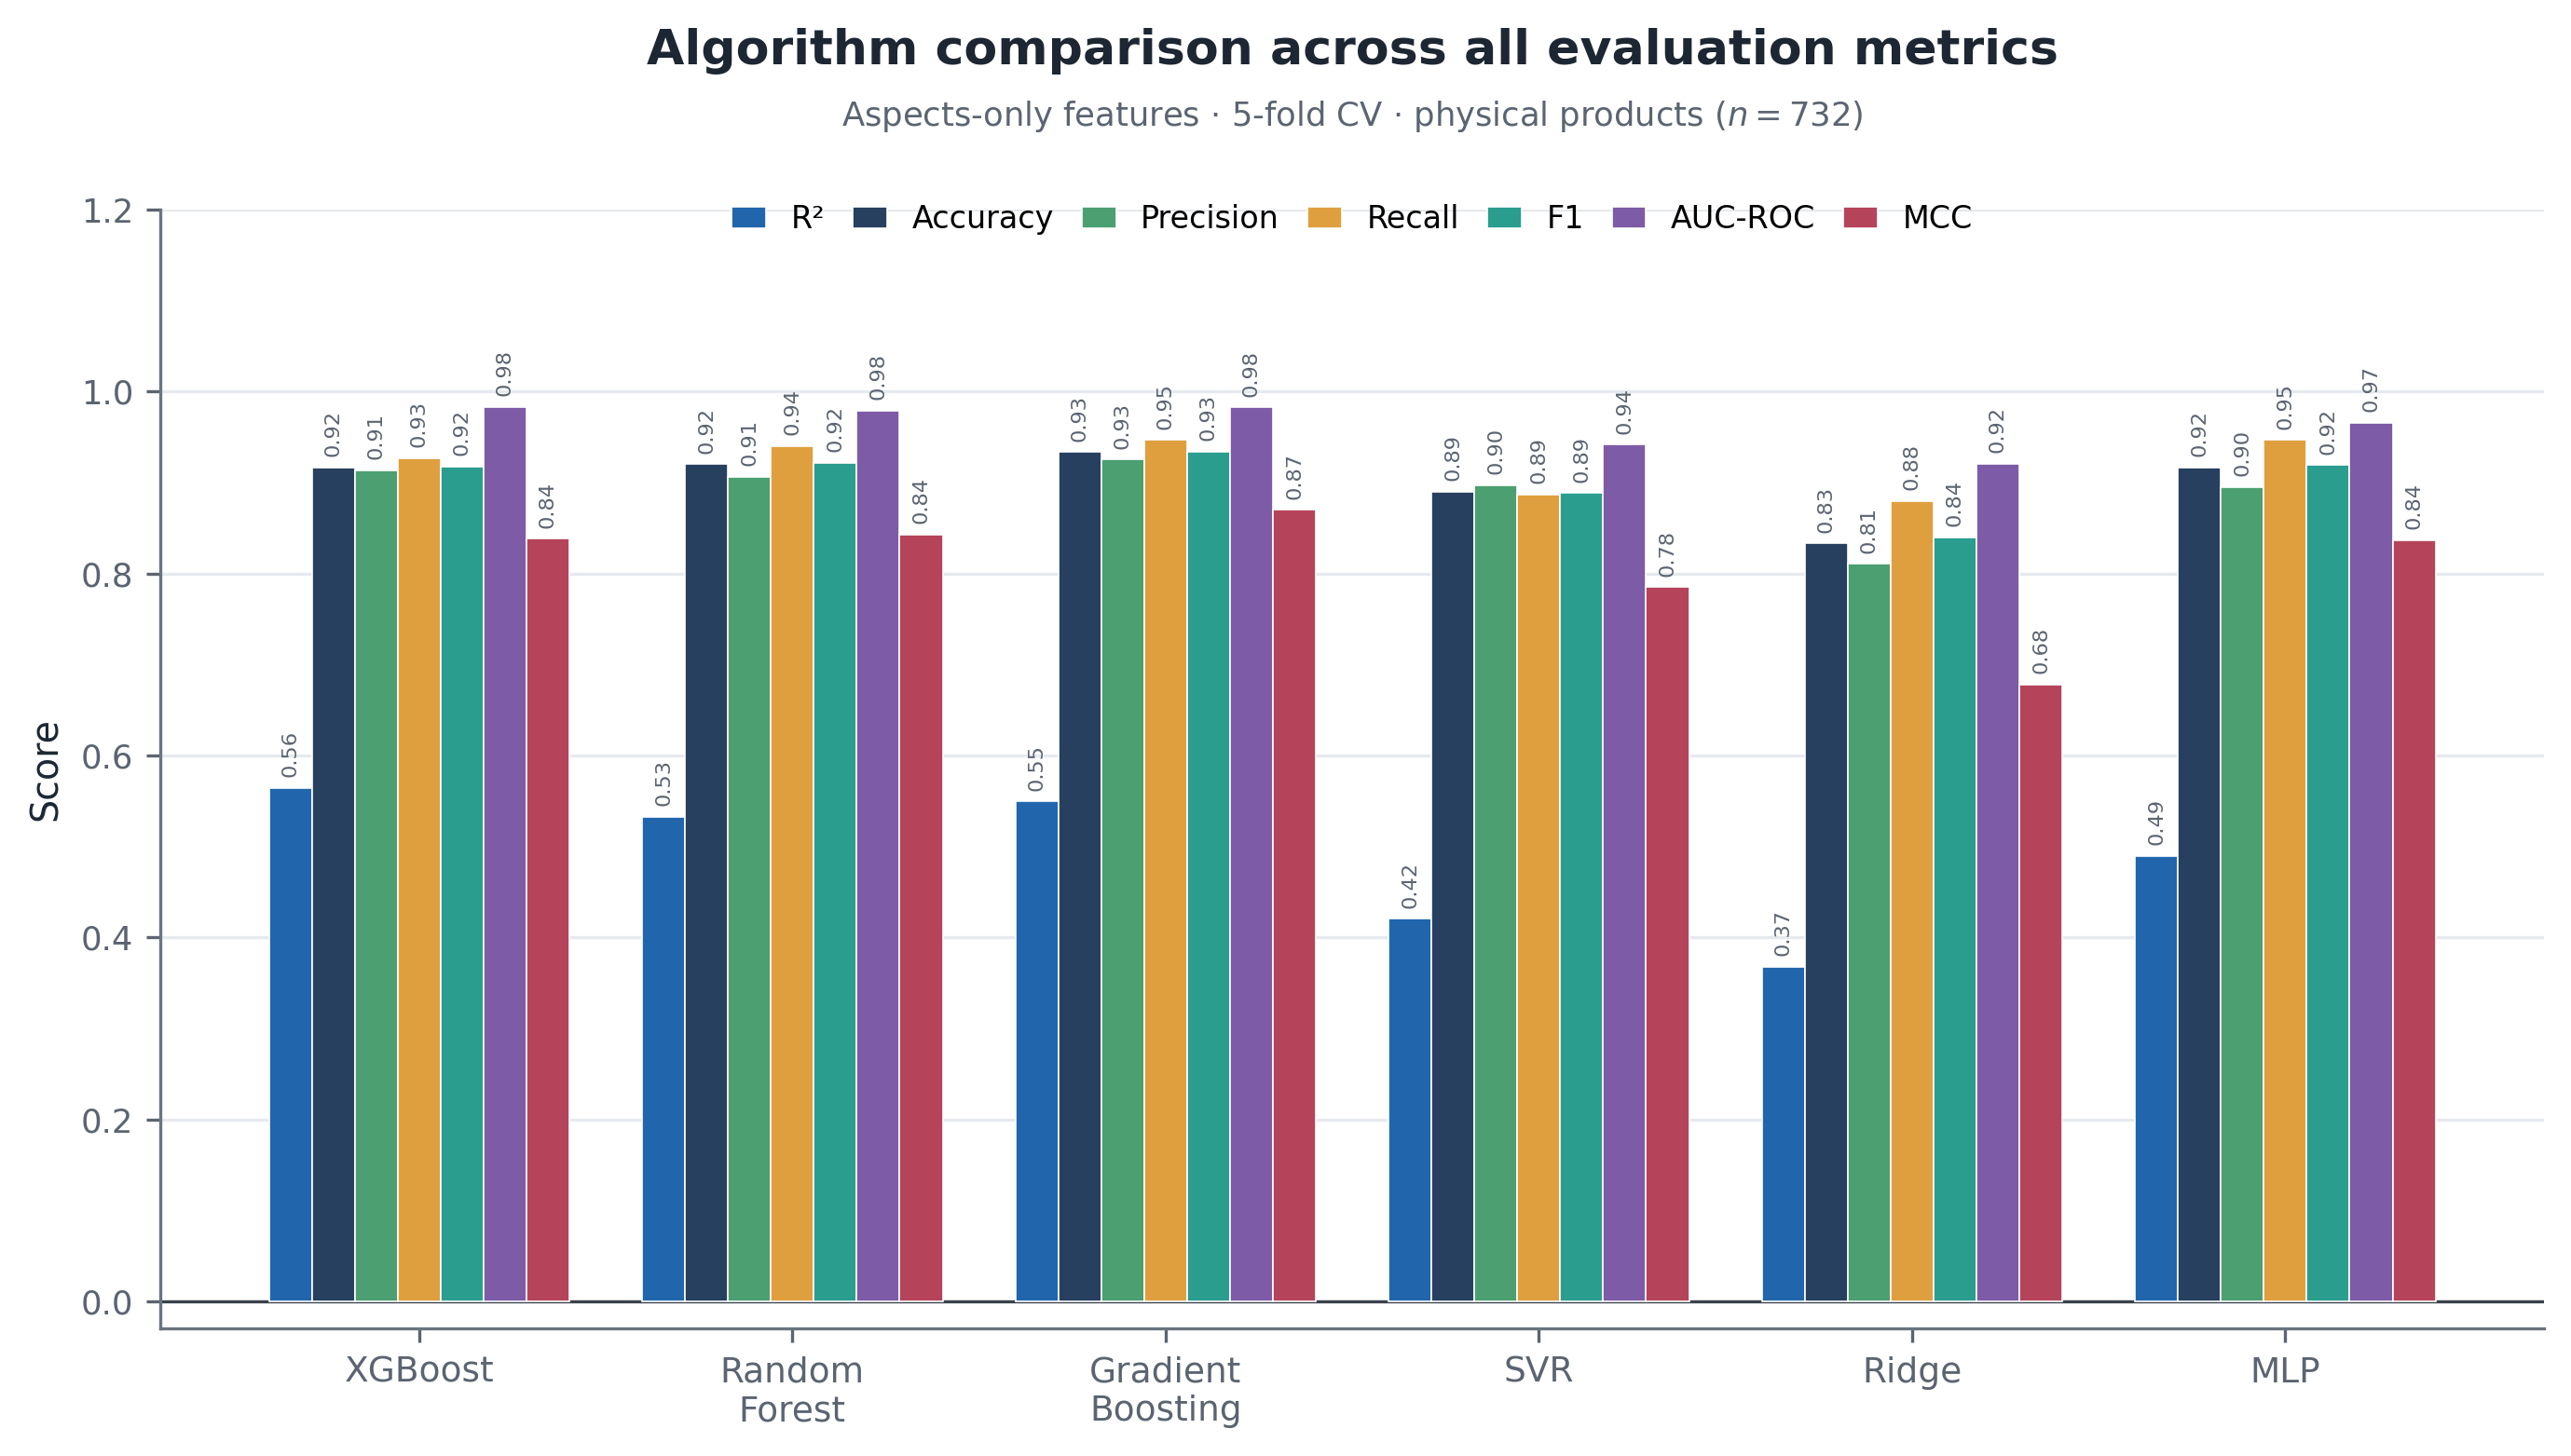
\includegraphics[width=\columnwidth]{fig7_algorithm_metrics.png}
\caption{All evaluation metrics across six algorithms on the aspects-only feature set (5-fold CV, $n=732$). Metrics: $R^2$, Accuracy, Precision, Recall, F1, AUC-ROC, and MCC.}
\label{fig:algometrics}
\end{figure}

\begin{figure}[!t]
\centering
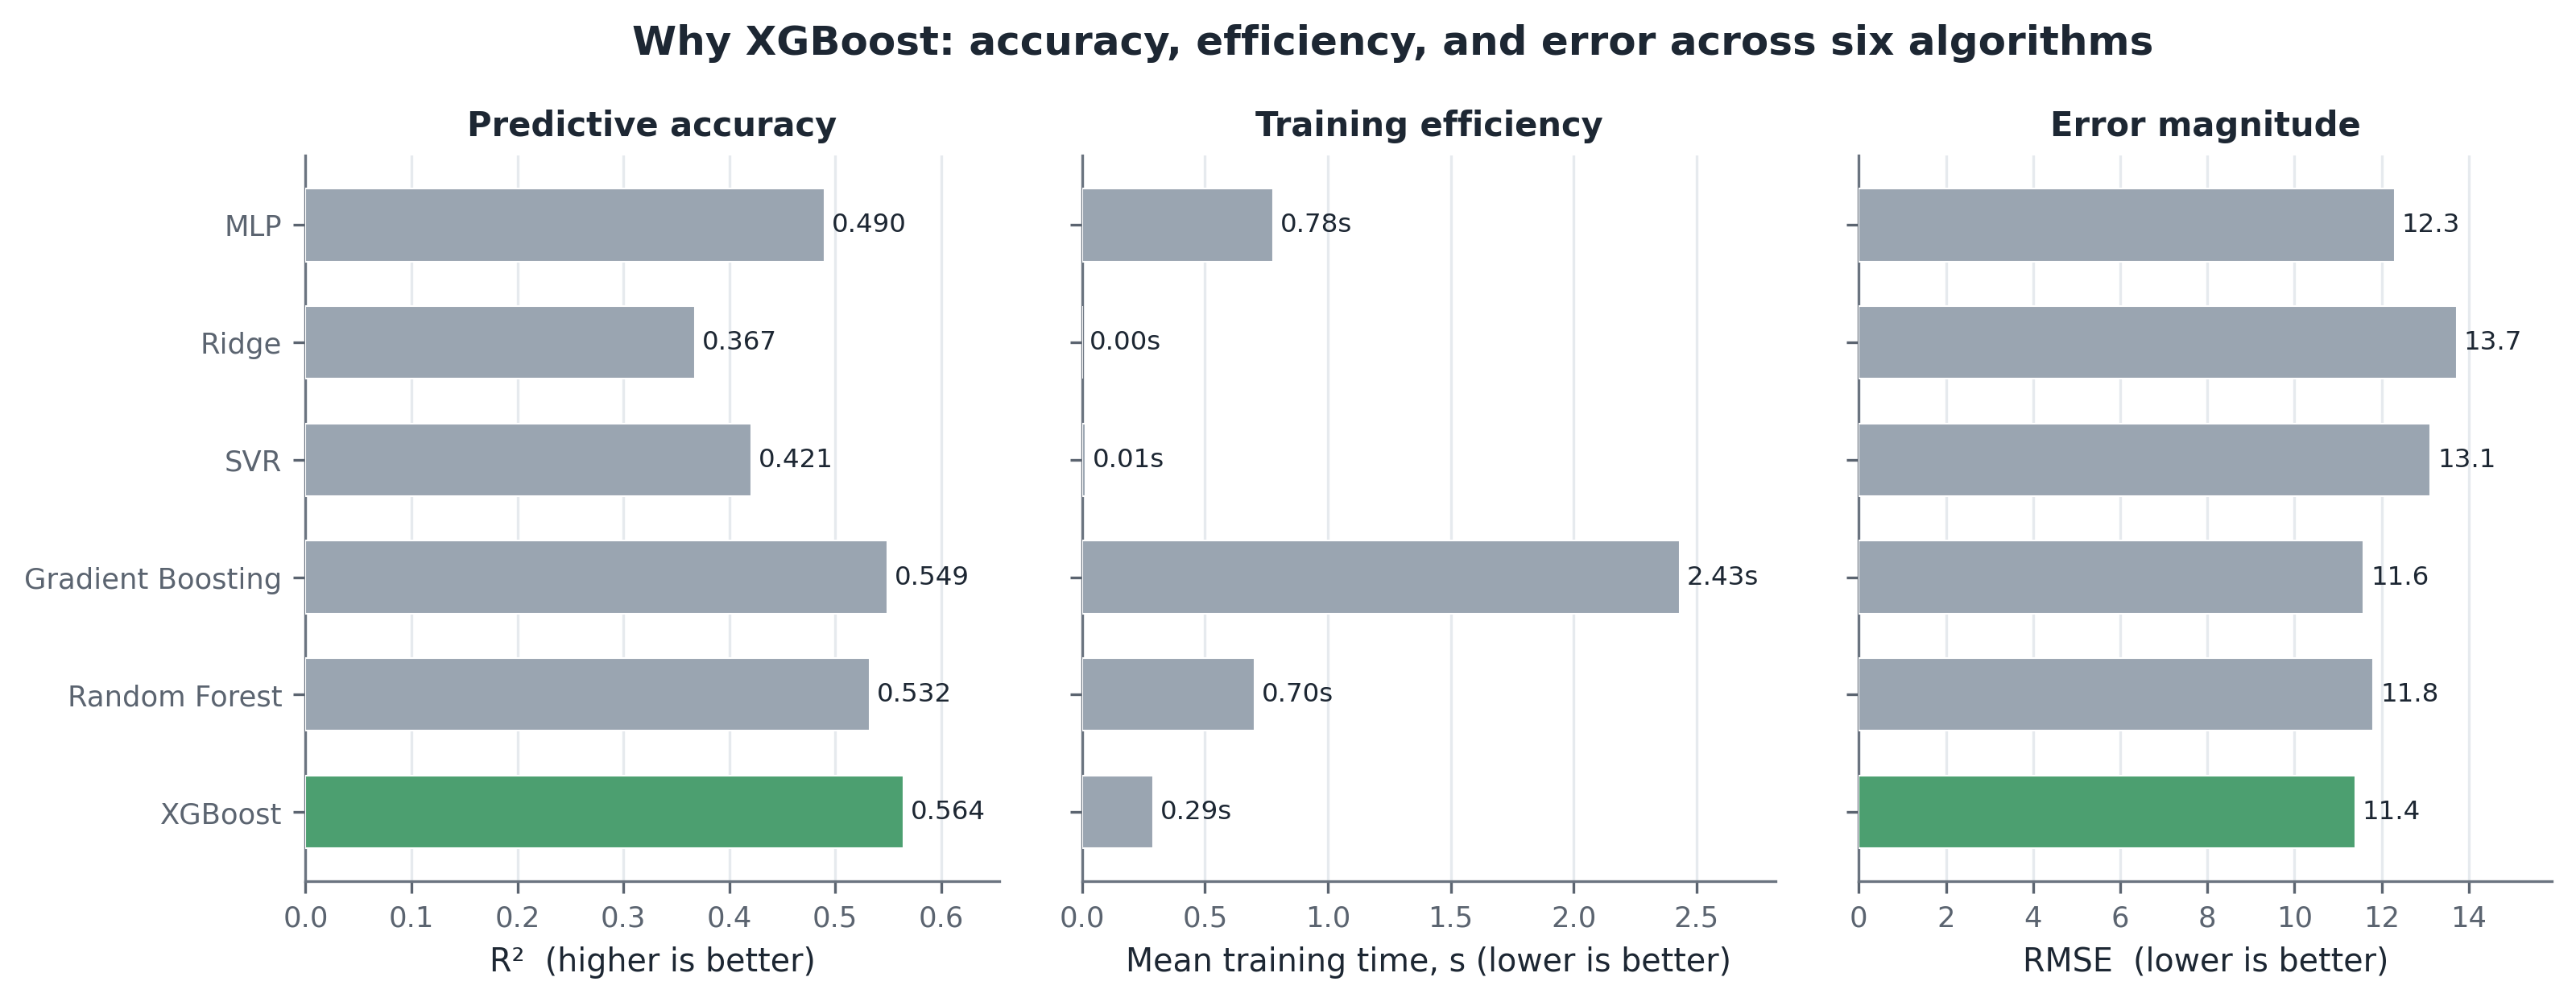
\includegraphics[width=\columnwidth]{fig8_algorithm_tradeoffs.png}
\caption{Three-panel accuracy--efficiency trade-off: predictive accuracy ($R^2$), training time, and error magnitude (RMSE). XGBoost leads on accuracy and error with competitive speed.}
\label{fig:algotradeoffs}
\end{figure}

\begin{figure}[!t]
\centering
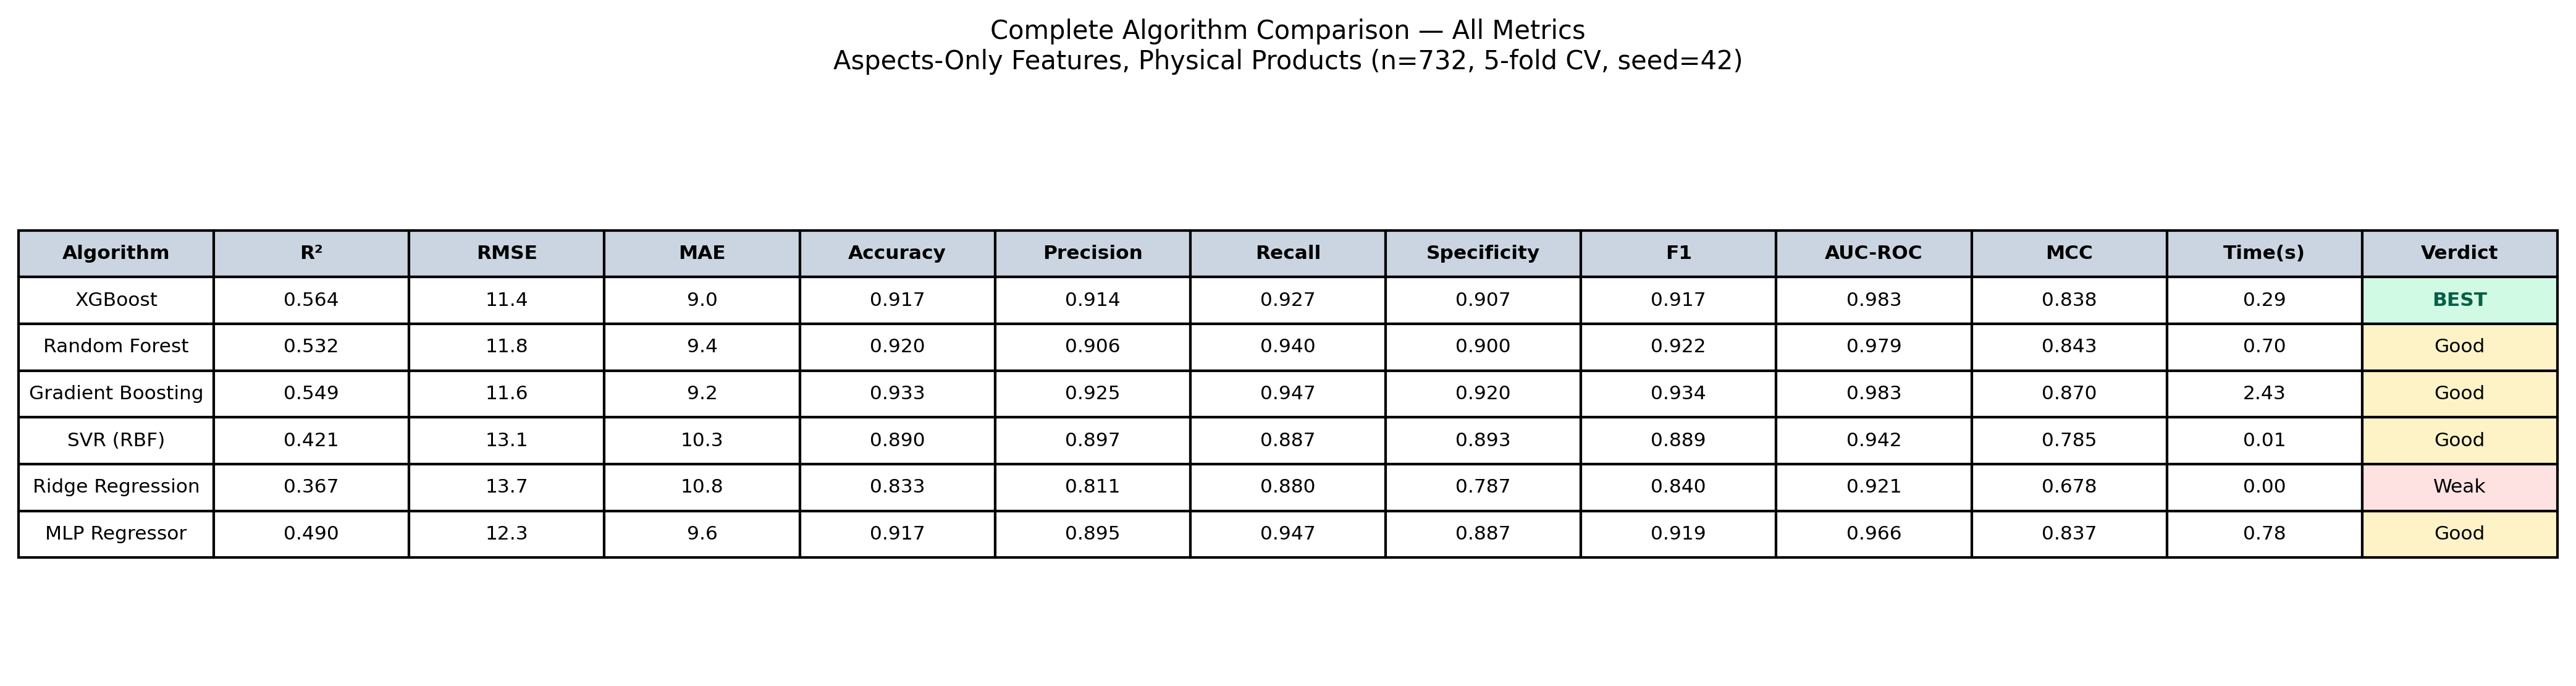
\includegraphics[width=\columnwidth]{fig9_algorithm_table.png}
\caption{Complete numerical comparison across all evaluation metrics. Bold verdict column summarises the overall ranking: XGBoost is the only algorithm rated BEST on both regression accuracy and classification-derived measures while maintaining competitive training time.}
\label{fig:algotable}
\end{figure}

\begin{figure}[!t]
\centering
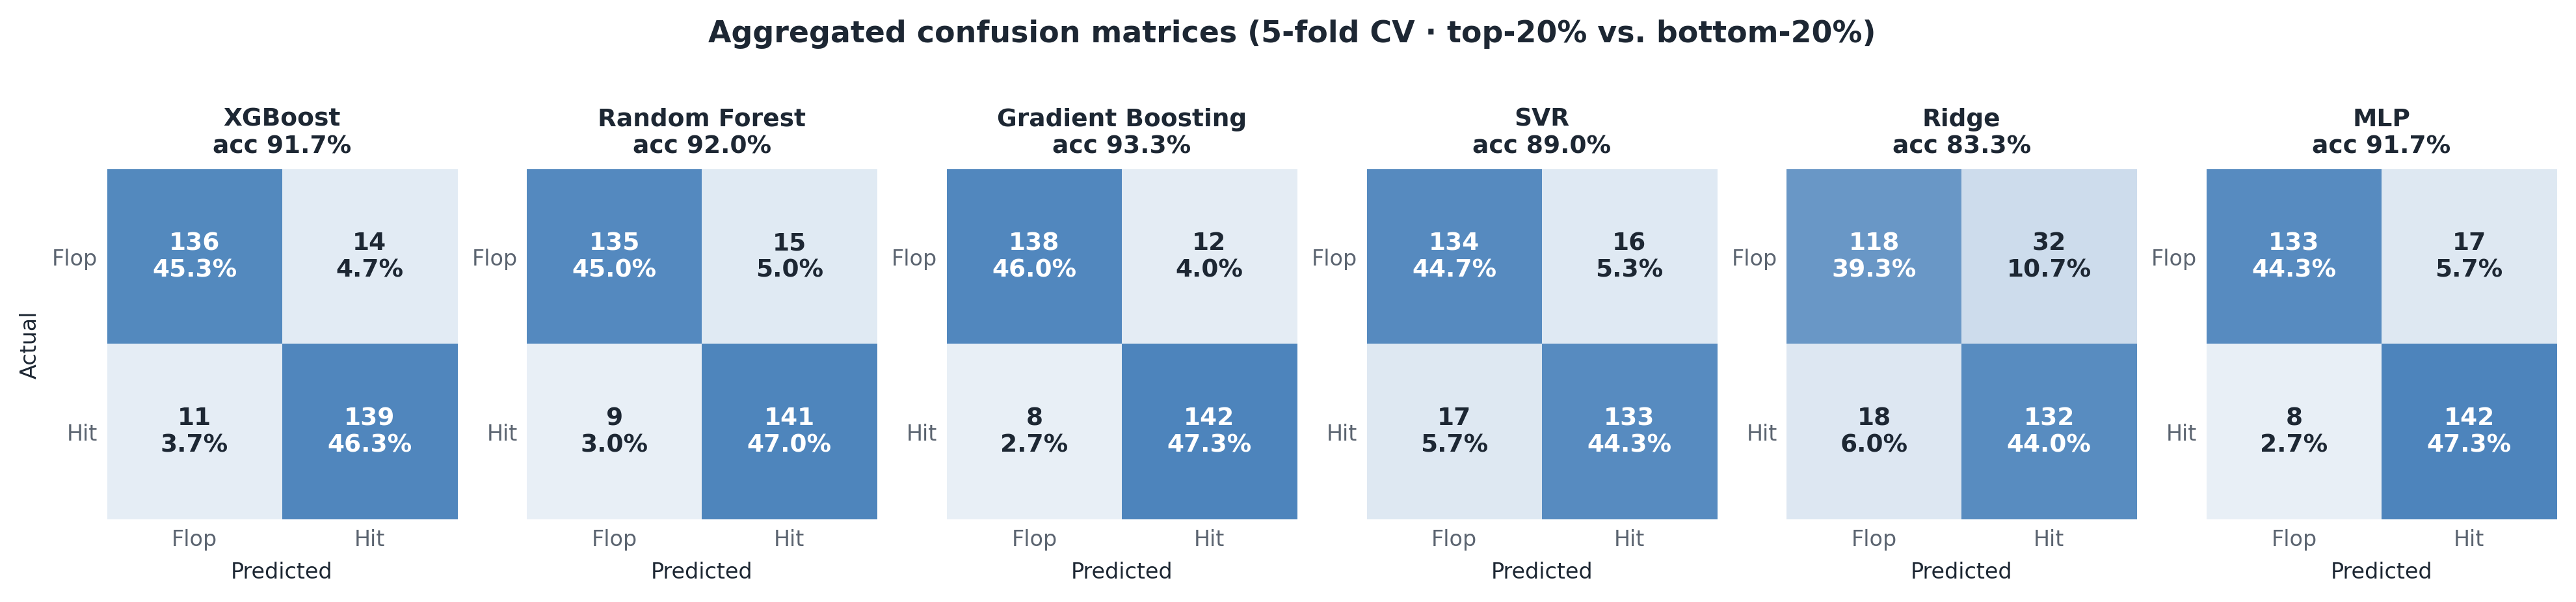
\includegraphics[width=\columnwidth]{fig10_confusion_matrices.png}
\caption{Aggregated confusion matrices (5-fold CV, top-20\% vs.\ bottom-20\% products). Counts and percentages for each quadrant: true negatives (flops correctly identified), false positives, false negatives, and true positives (hits correctly identified).}
\label{fig:confmat}
\end{figure}

\subsection{Bridging: Estimating Aspects from Specifications}
The bridging layer asks an LLM to estimate the aspect profile a product \emph{would} earn after months of real use, given only its specification and a category profile: price quartiles, mean aspect scores, and the top pain points and strengths mined from real reviews, plus the community priorities of Section~\ref{sec:reddit} when they are available. Our first prompt trusted its input, and it failed in a useful way. Marketing copy is optimistic by design, promoting flops and hits with the same enthusiasm, and the predictions collapsed into a narrow optimistic band. The production prompt (v2) rests on three skeptic rules. Under \emph{adjective blindness}, only verifiable facts can justify a score, meaning materials, standards, numbers, and warranty terms: ``powerful bass'' is noise, while ``50\,mm drivers'' is evidence. Under the \emph{absence rule}, a spec that offers no concrete evidence for an aspect is treated as a signal in itself, since a competent team states its strengths, so the aspect is scored below the category mean and flagged as ungrounded. Under \emph{anchor discipline}, the category mean is what the median real product achieves, and any score more than two points above it has to cite a spec fact. Section~\ref{sec:validation} quantifies the effect ($\rho$ $0.241 \to 0.313$, AUC $0.653 \to 0.761$; Fig.~\ref{fig:ablation}) and rules out a verbosity confound with a partial correlation.

\subsection{The Honesty Layer}
Bridged estimates are more reliable for some aspects than others, and the system shows that measured validity rather than hiding it. Each aspect carries a trust badge taken from the retrospective validation (Fig.~\ref{fig:validity}): STRONG (utility, ease of use, build quality), MODERATE (value for money, reliability, durability), or NO SIGNAL (design appeal, after-sales, repairability). When at least half the aspects are ungrounded, an abstention banner appears and points the user to the spec coach instead of to a number. Viability is shown as a $\pm 5$ range, because a single decimal would claim a precision the validation does not support, and it is placed next to a percentile rank against the 90 retrospectively bridged real products.

\begin{figure}[!t]
\centering
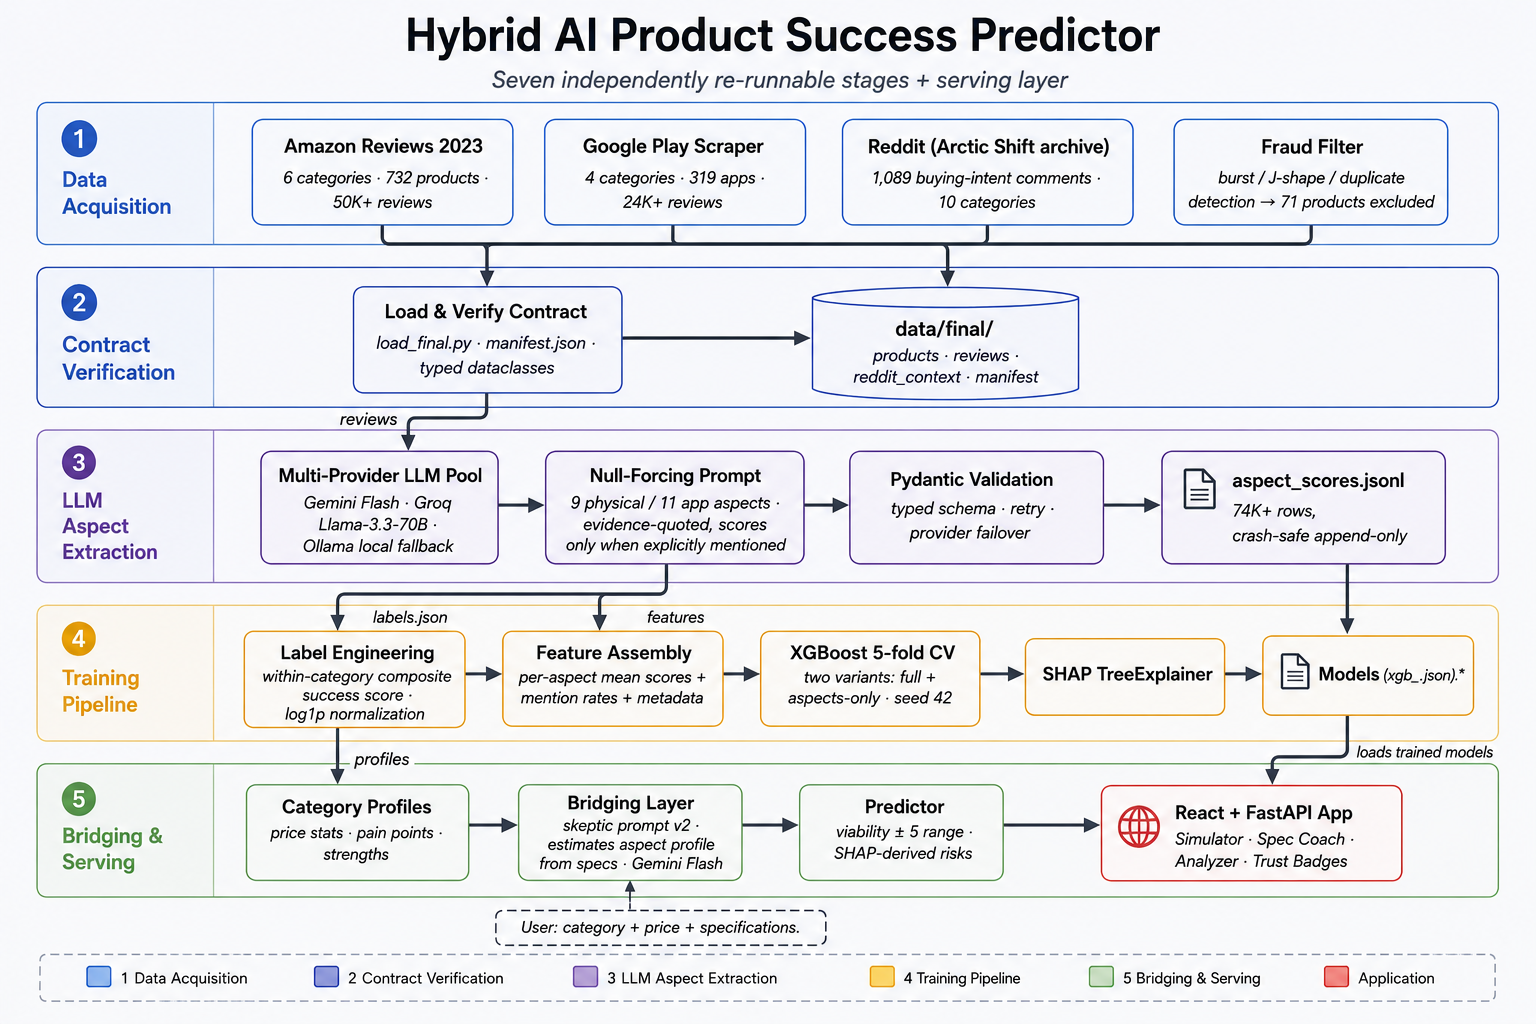
\includegraphics[width=\columnwidth]{fig1_pipeline.png}
\caption{Pipeline overview: extraction, label engineering, feature assembly, training, category profiling, and the bridging/prediction service.}
\label{fig:pipeline}
\end{figure}

\section{Validation}
\label{sec:validation}

\subsection{Retrospective Launch-Blind Harness}
The central validation question is a counterfactual: \emph{had our system existed on the day a real product launched, would its specs-only estimate have anticipated that product's eventual market outcome?} We answer it retrospectively. From the 732 physical products we drew a stratified sample of 90, three per (category $\times$ success-quintile) cell, so that flops and hits appear in equal numbers rather than in their natural, success-skewed proportions.

For each sampled product, the bridging layer saw only what was knowable at launch: name, brand, price, and the manufacturer's marketing copy. Reviews, ratings, and sales signals were withheld. The bridged profile went into the aspects-only model, and its estimate was compared against the product's actual success score, computed from the thousands of reviews it later accumulated. One caveat we note rather than bury: the category profiles include each target product's own reviews at roughly $1/130$ weight. We judge this leakage negligible, but it is there.

On this 90-product development set the pipeline reached Spearman $\rho = 0.313$ ($p = 0.003$), Pearson $r = 0.361$, and a flop-versus-leader AUC of 0.761, computed between the top and bottom actual-success quintiles. Mean predicted viability climbed monotonically across all five quintiles ($59.1 \to 61.1 \to 61.4 \to 63.2 \to 65.7$), a spread of 6.6 points.

\subsection{Pre-Registered Confirmatory Holdout}
Every design decision above was tuned on the same 90 products, which is a textbook overfitting risk. So we pre-registered a confirmatory study \cite{nosek2018preregistration}. Before the run, we drew 59 products disjoint from the development set (fixed seed), froze the entire pipeline, and pre-specified the analysis. Nothing was tuned after we saw the result.

The holdout reproduced the development findings: $\rho = 0.317$ ($p = 0.014$), with a bootstrap 95\% CI of $[0.059, 0.543]$ that excludes zero; AUC $= 0.743$, CI $[0.51, 0.93]$; and tier means that are again strictly monotonic ($58.5 \to 60.8 \to 61.7 \to 62.8 \to 64.1$; Fig.~\ref{fig:holdout}). The point estimates land within a few thousandths of the development values, which is what a real signal looks like and a tuned artifact usually does not. We treat this pre-registered replication as the paper's primary evidence, and we give the interval as much weight as the point estimate. At $n = 59$, $\rho = 0.317$ explains on the order of 10\% of the rank variance. That is a screening signal for a portfolio of candidate designs, not a verdict on any one product.

\begin{figure}[!t]
\centering
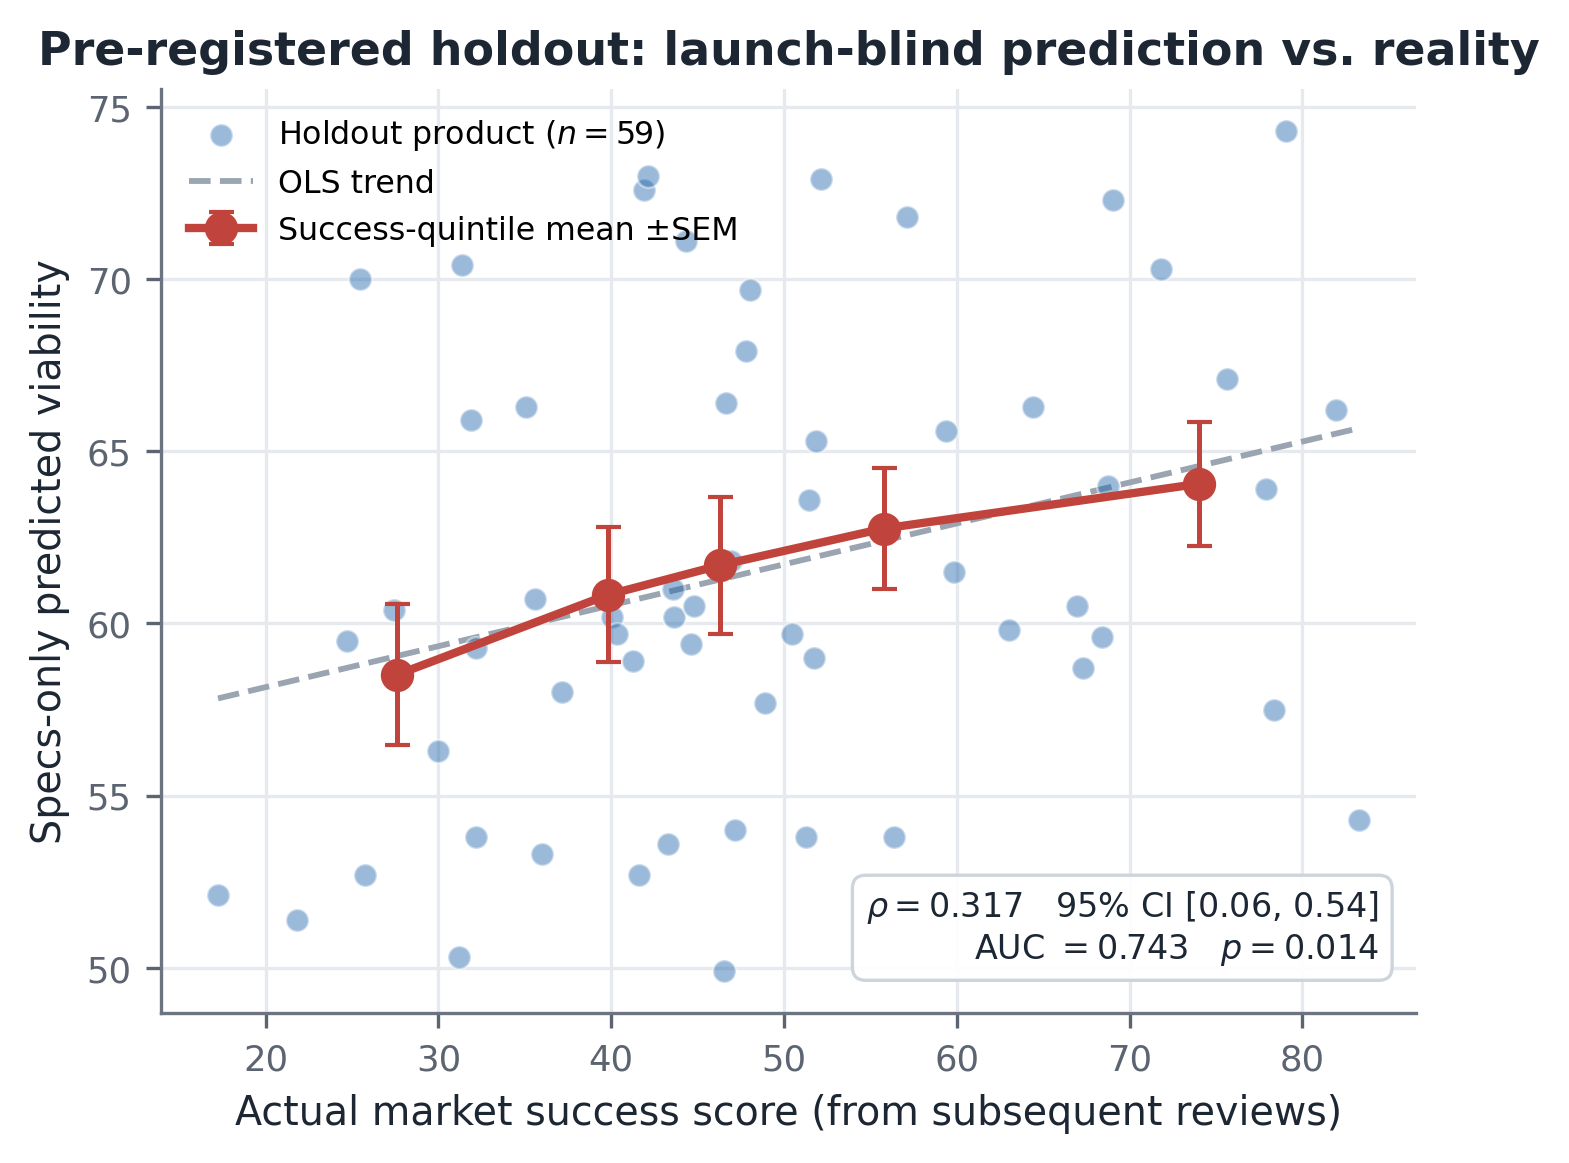
\includegraphics[width=\columnwidth]{fig2_holdout_scatter.png}
\caption{Pre-registered holdout ($n=59$): specs-only predicted viability versus actual market success, with monotonic success-quintile means.}
\label{fig:holdout}
\end{figure}

\subsection{Baselines, Ablations, and Rejected Alternatives}
A launch-blind correlation only matters if it is not just rediscovering something trivial. Three baselines use the same launch-knowable inputs: price-distance from the category median gives $\rho = -0.178$; marketing-copy length gives $\rho = -0.259$, so longer copy weakly signals \emph{worse} outcomes; and the strongest baseline, within-category price percentile, gives $\rho = 0.250$. The full pipeline beats that baseline only modestly in magnitude, but the two signals are almost orthogonal ($r = 0.135$). The pipeline is not re-deriving price position, and a post-hoc rank ensemble of the two reaches $\rho = 0.320$, which we report as exploratory.

Two ablations shaped the final system (Fig.~\ref{fig:ablation}). We kept the skeptic prompt, which raised $\rho$ from 0.241 to 0.313 and AUC from 0.653 to 0.761 on identical products; a partial correlation controlling for spec length shows the lift is not a verbosity proxy ($\rho = 0.303$, $p = 0.004$). We dropped validity-weighted shrinkage toward the category means. Intuition strongly favored it, but a leave-one-out evaluation showed it \emph{lowers} $\rho$ from 0.313 to 0.249, apparently by destroying the cross-aspect covariance the downstream model relies on. We keep it in the paper as a cautionary result: a plausible calibration step still has to be tested with held-out weights before it ships.

\begin{figure}[!t]
\centering
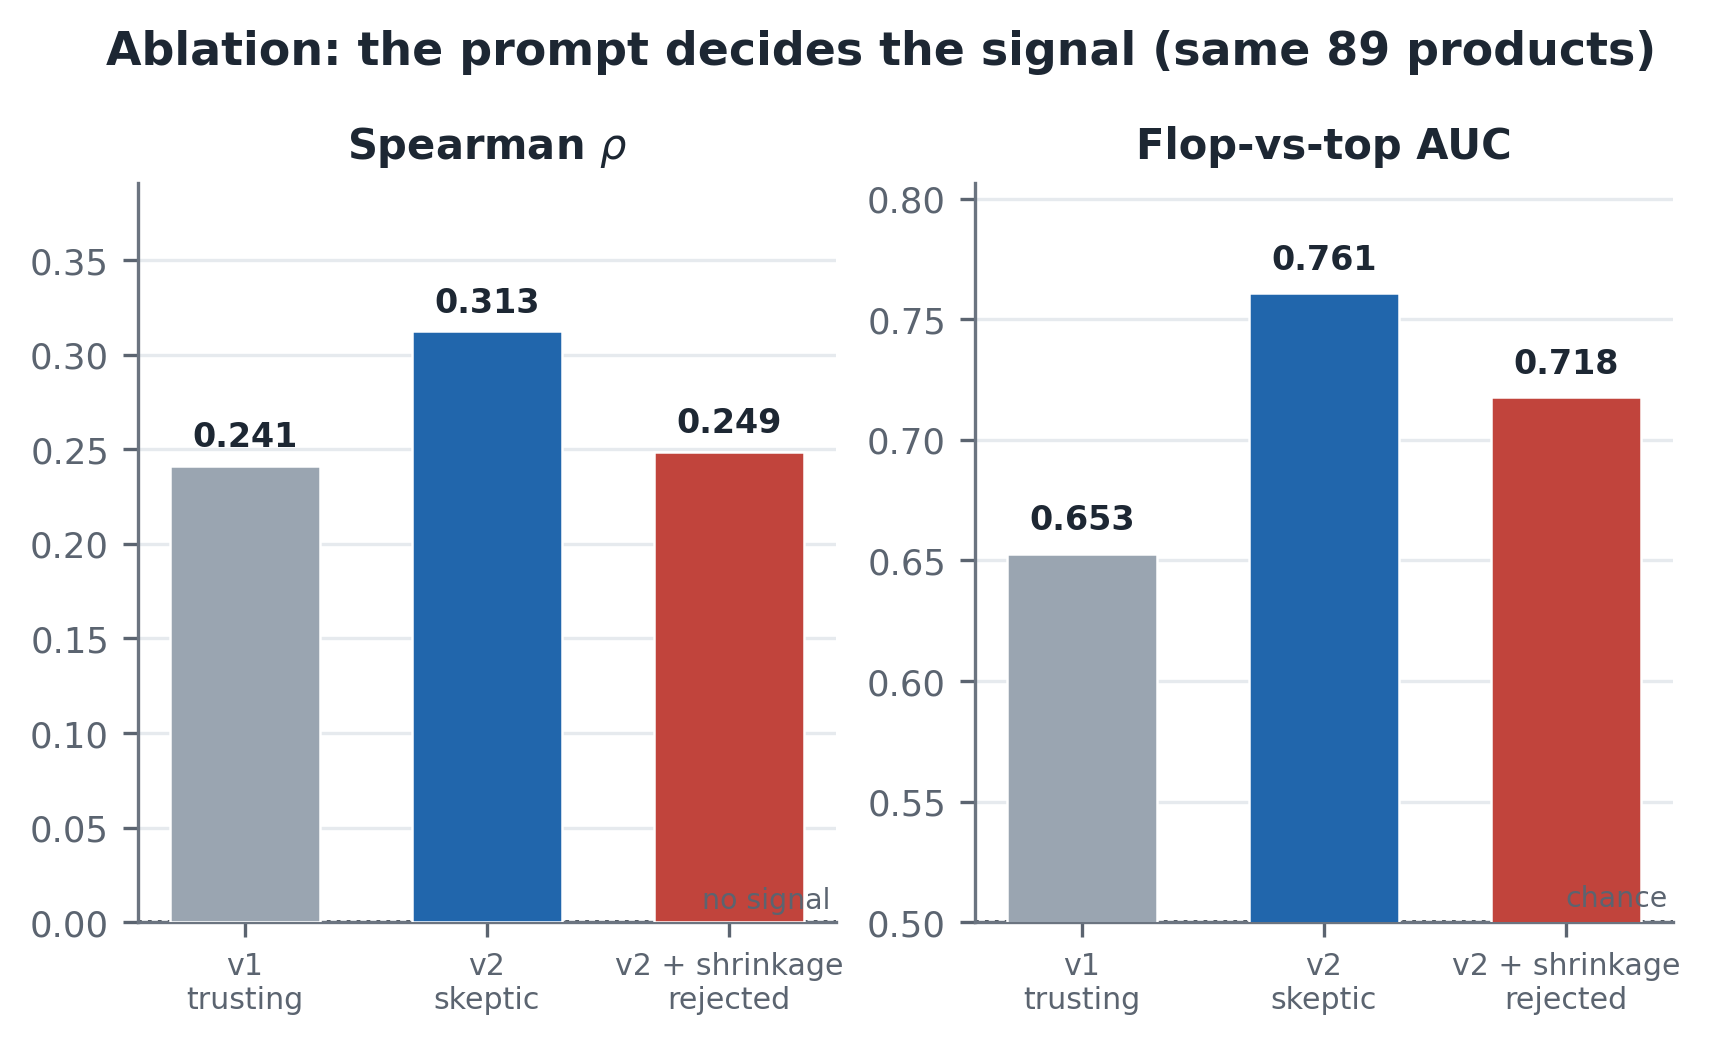
\includegraphics[width=\columnwidth]{fig4_prompt_ablation.png}
\caption{Ablation on identical products: trusting prompt (v1), skeptic prompt (v2), and the rejected shrinkage variant.}
\label{fig:ablation}
\end{figure}

\subsection{Which Aspects Can Be Estimated from Specs}
Per aspect, the bridged estimates correlate with review-derived ground truth at $r = 0.44$ $[0.23, 0.61]$ for ease of use, $0.40$ $[0.20, 0.58]$ for build quality, $0.39$ for durability and reliability, $0.38$ for utility, and $0.33$ for value for money. At the other end, after-sales ($r = 0.05$ $[-0.18, 0.28]$) and design appeal ($r = 0.19$) are essentially unestimable from a specification (Fig.~\ref{fig:validity}). That makes sense: service quality is invisible on a spec sheet, and aesthetics are subjective in a way category norms do not capture. The application shows these tiers verbatim as trust badges. On the holdout the per-aspect correlations broadly hold up (ease of use 0.53, utility 0.51), with one honest exception: build quality dropped to $r = 0.13$, which we flag as an instability to investigate rather than smooth over.

\begin{figure}[!t]
\centering
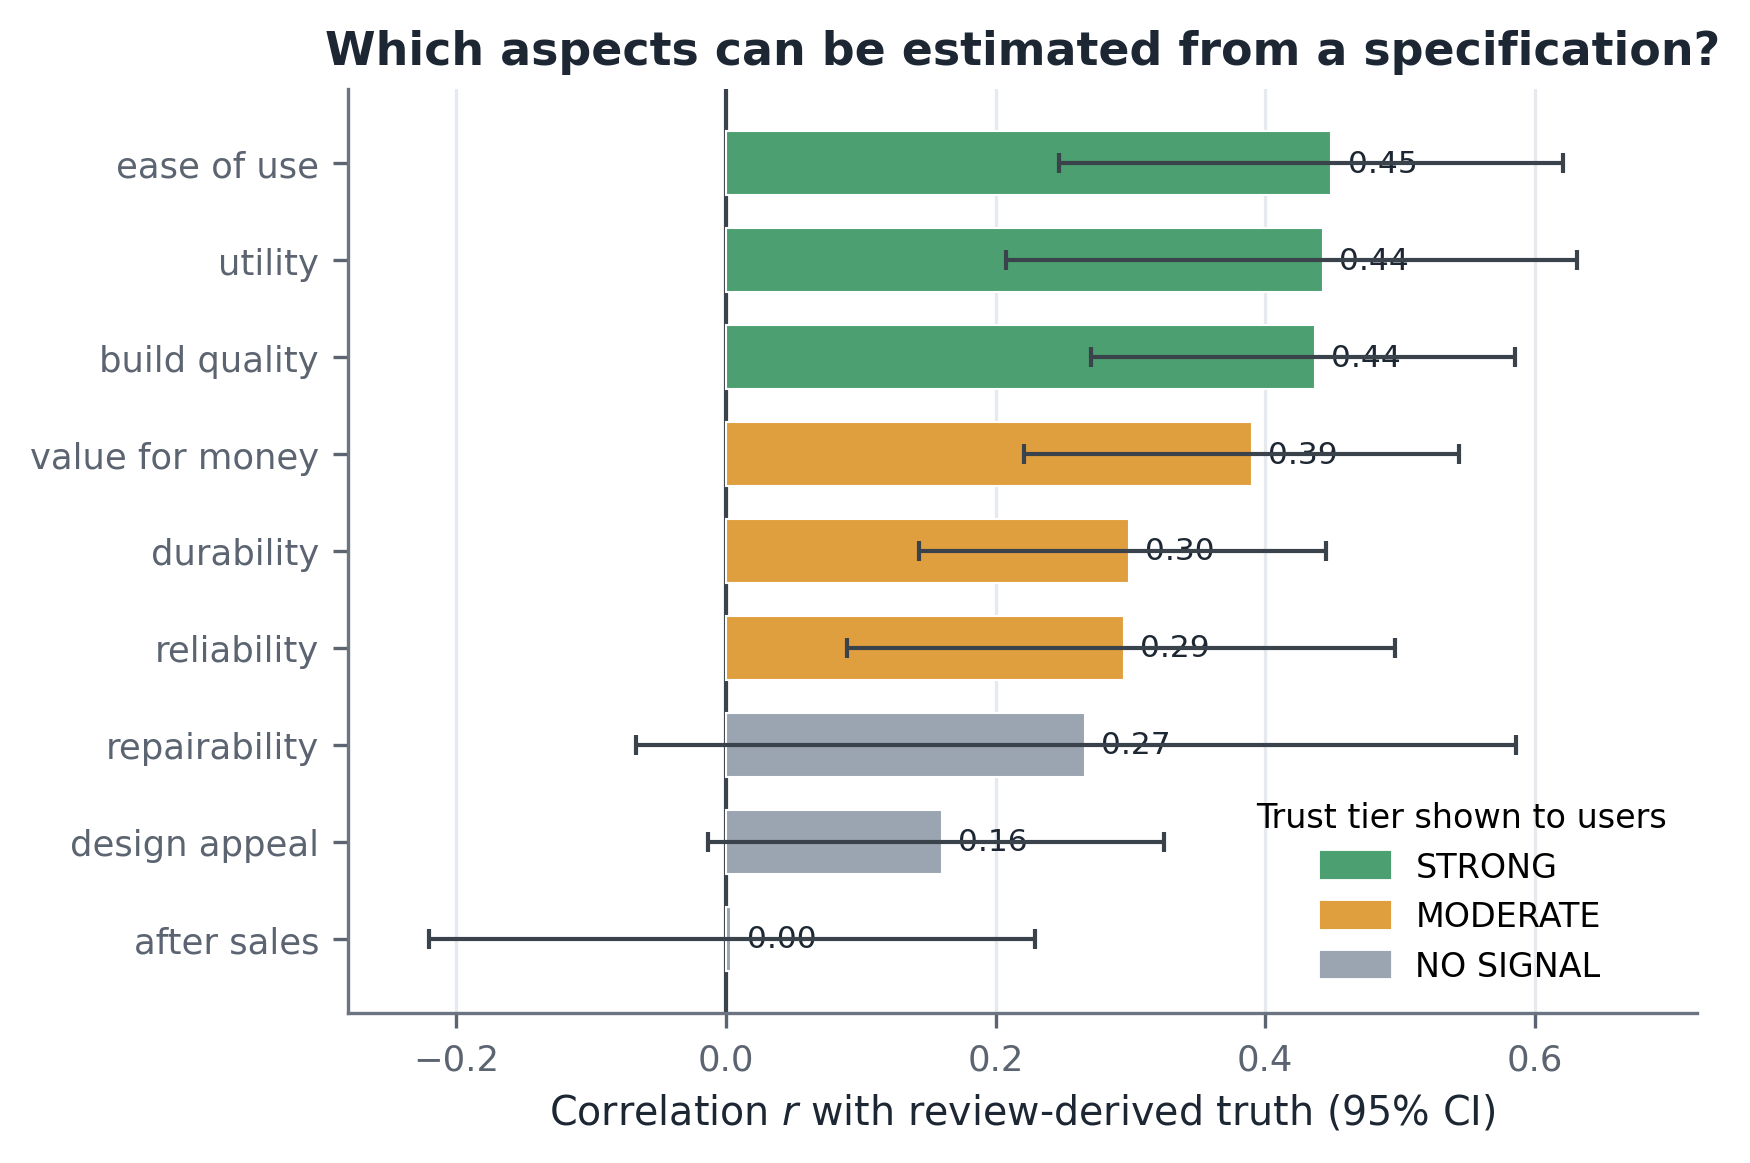
\includegraphics[width=\columnwidth]{fig3_aspect_validity.png}
\caption{Per-aspect validity of bridged estimates (r with 95\% CI), colored by the trust tier shown to users.}
\label{fig:validity}
\end{figure}

\subsection{Named-Product Spectrum}
As a face-validity check, we looked at the ranked spectrum by name. The top of the specs-only predictions holds products that went on to gather 30{,}000--78{,}000 ratings (established Bose, JBL, and DOSS lines); the bottom holds a smartwatch clone that ended up with a 2.9-star average. Seeing nothing but launch copy, the system gets the extremes of the market right. The middle stays noisy, which is exactly what the $\rho$ already told us.

\section{Negative Finding: The Mobile-App Track}
\label{sec:negative}
We built the pipeline symmetrically for physical products and mobile applications, and for applications it fails. We report that with the same prominence as the successes. Against our pre-registered acceptance gate (CV $R^2 \geq 0.35$ for the aspects-only model), the app track scores $R^2 = 0.101$ ($n = 319$). The full model reaches $R^2 = 0.889$, but only by leaning on install counts and rating volume, which are post-launch popularity metadata a pre-production tool cannot have.

The obvious rescue hypothesis is that the \emph{target} is at fault. Our composite weights installs and velocity at 50\%, and those are distribution outcomes driven by marketing spend, store placement, and network effects, none of which product quality can see. If that were the whole story, review aspects should still predict the quality-side outcomes. We tested it directly, retraining the identical aspects-only model against five outcome definitions under the same cross-validation: the composite ($R^2 = 0.101$), average rating (0.153), a retention proxy ($-0.012$), normalized installs (0.231), and review velocity (0.072). None comes near the gate (Fig.~\ref{fig:apptargets}). The most telling result is that review aspects cannot predict even an app's \emph{own average rating}. So the failure is not an artifact of how we defined the target; it is more basic than that. App-store ratings are squeezed into a narrow 4.0--4.6 band, the categories we studied are dominated by free apps whose review sentiment circles monetization and advertising rather than durable quality, and success is distribution-driven from end to end.

Two conclusions follow. As a method, the framework doubles as an instrument for finding out \emph{which} market outcomes are learnable from quality signals: physical-product success partly is, and app-store success, under every definition we tried, is not. In practice, we retired the app track from the tool's user-facing surface. The option is still visible but disabled, with the experiment cited, because quietly deleting a failed track would misrepresent what we actually attempted.

\begin{figure}[!t]
\centering
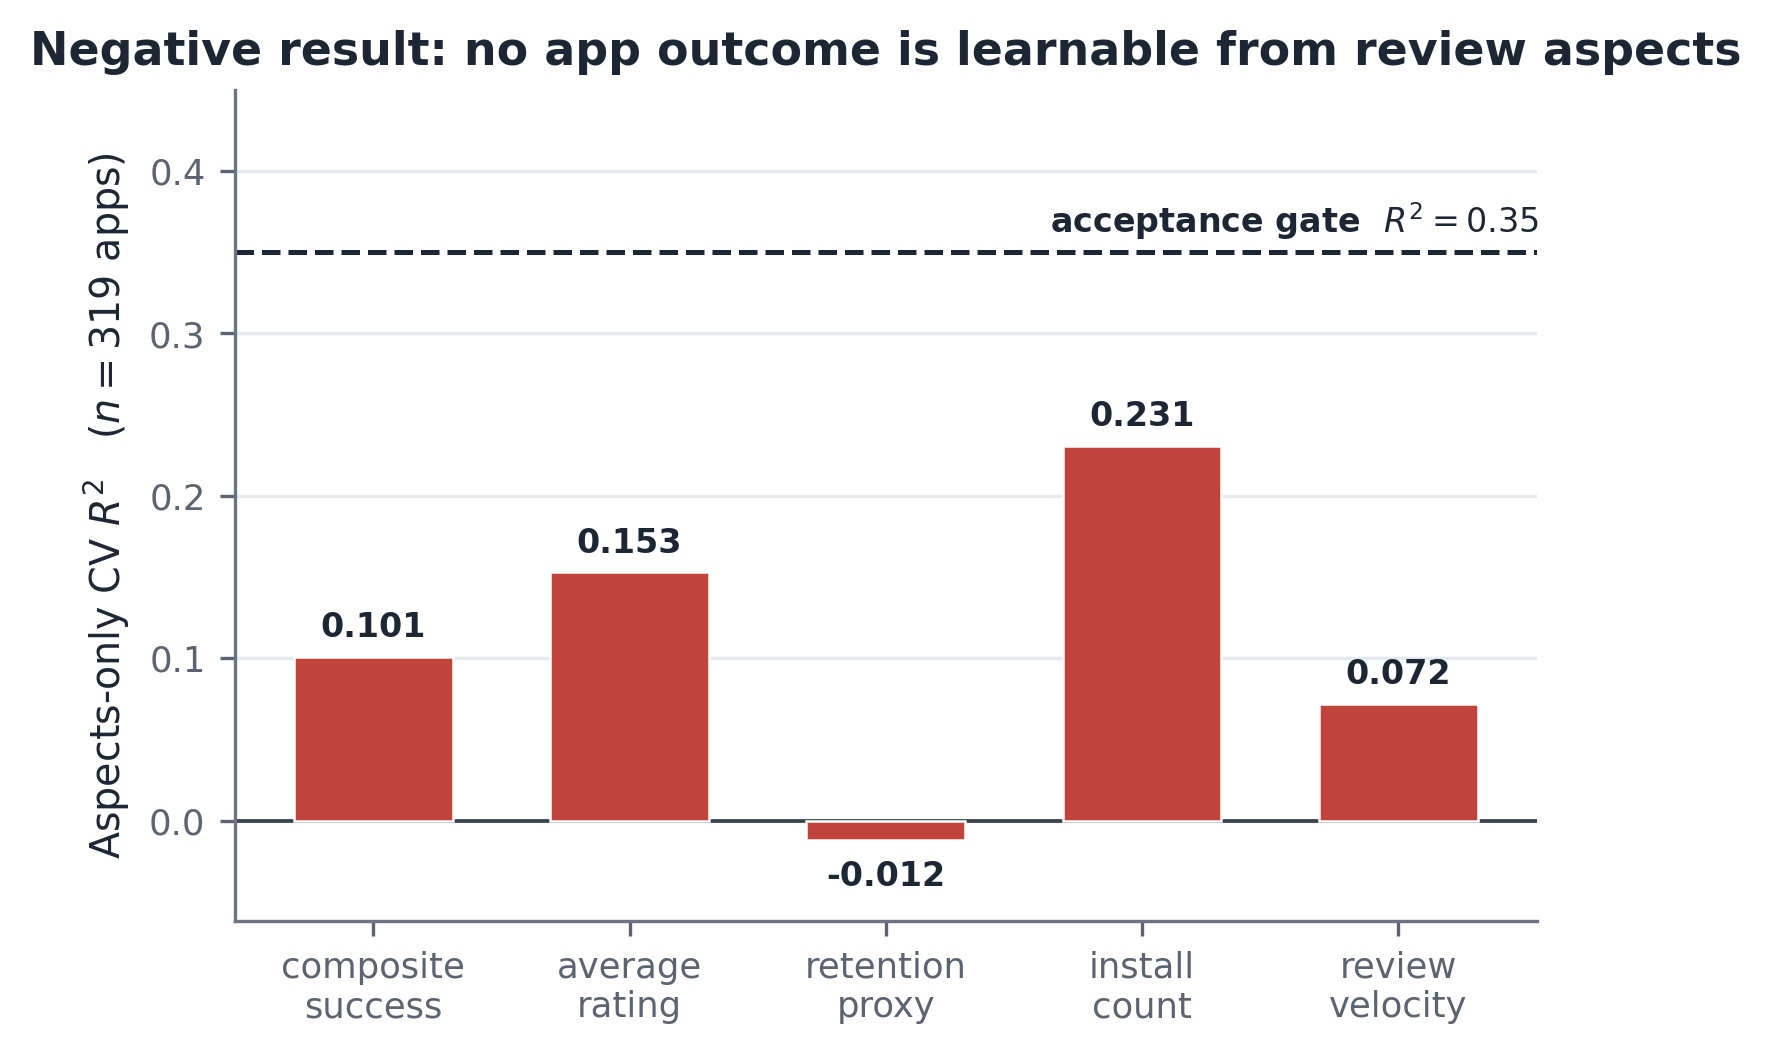
\includegraphics[width=\columnwidth]{fig5_app_target_sweep.png}
\caption{Five-target sweep for mobile applications: no outcome definition is learnable from review aspects.}
\label{fig:apptargets}
\end{figure}

\section{Exploratory: Community Priors}
\label{sec:reddit}
Category profiles ground the bridging prompt in review-derived statistics, but reviews describe products people already bought. Community discussions capture something else: what buyers \emph{wish they had known} first. We collected 1{,}089 buying-intent comments across all ten categories (Section~\ref{sec:data}), summarized each category's consumer priorities with a single LLM call, and fed that summary into the bridging prompt.

We measured the effect with a paired A/B. The same 89 development products were bridged twice with the same provider and seed, differing only in whether the priorities field was present. With priorities, $\rho$ rose from 0.311 to 0.359 and AUC from 0.728 to 0.752. But the paired bootstrap 95\% CI on the $\rho$ difference is $[-0.025, +0.125]$, and it includes zero, so \textbf{we report the lift as suggestive, not confirmed.} This comparison, unlike the holdout of Section~\ref{sec:validation}, was not pre-registered. Two things put it in context. The without-priorities arm reproduces the original baseline on its own (0.311 against 0.313), which says the harness is stable; and the input was small, about a thousand comments with tails as thin as 18 for smartphones, so if the effect is real its data-efficiency would be worth a closer look. Confirming it, ideally with a pre-registered replication on the holdout, is future work.

\section{System}
\label{sec:system}
The pipeline runs as seven independently re-runnable stages (Fig.~\ref{fig:pipeline}). Each stage writes its output to disk and skips expensive work unless forced to redo it. The extraction stage is crash-safe and resumable, which mattered in practice, because the full batch runs for days of rate-limited API calls across a rotating provider pool. Feature manifests are serialized to disk, and the prediction code builds its input vectors by iterating over them, so the serving path can never quietly drift out of alignment with training. A single end-to-end smoke test regenerates synthetic data and runs every stage in a sandbox, and it gates every code change.

The user-facing application (Fig.~\ref{fig:ui}a) is a React front end on a FastAPI backend. A founder describes a product by category, price, and free-text specification, and gets the full analysis back: a viability range (deliberately $\pm 5$ wide), a percentile rank against the 90 retrospectively bridged real products, per-aspect estimates plotted against category averages, SHAP-derived \cite{lundberg2017shap} top risks and strengths stated in terms of design levers the founder actually controls, and a market-gap report that quotes verbatim customer complaints for the category pain points the design does not convincingly address. Every aspect estimate carries its trust badge and grounding flag, and when at least half the aspects are ungrounded, an abstention banner replaces the number with a redirect to the spec coach.

The spec coach (Fig.~\ref{fig:ui}b) closes the loop for users who are not practiced spec writers. One LLM call rates the draft's coverage of each aspect as covered, vague, or missing, asks at most five questions ordered by how much each answer would sharpen the prediction (favoring aspects that are both missing and top category pain points), and rewrites the spec while keeping every stated fact and inserting explicit placeholders for the decisions still to be made. The coach is forbidden, by construction, from inventing any material, number, or feature the user did not state.

Finally, the model-performance view (Fig.~\ref{fig:ui}c) renders the training report straight from its JSON artifact, including the mobile-application aspects-only row with its FAIL badge. Putting the system's own failed benchmark in the product UI, next to the disabled app-track option, is a deliberate choice, and it aligns with recent calls for calibrated autonomy in AI-assisted decisions \cite{cristofaro2026dancing}: a decision-support tool earns trust by showing where its competence ends as plainly as it shows where it works.

\begin{figure}[!t]
\centering
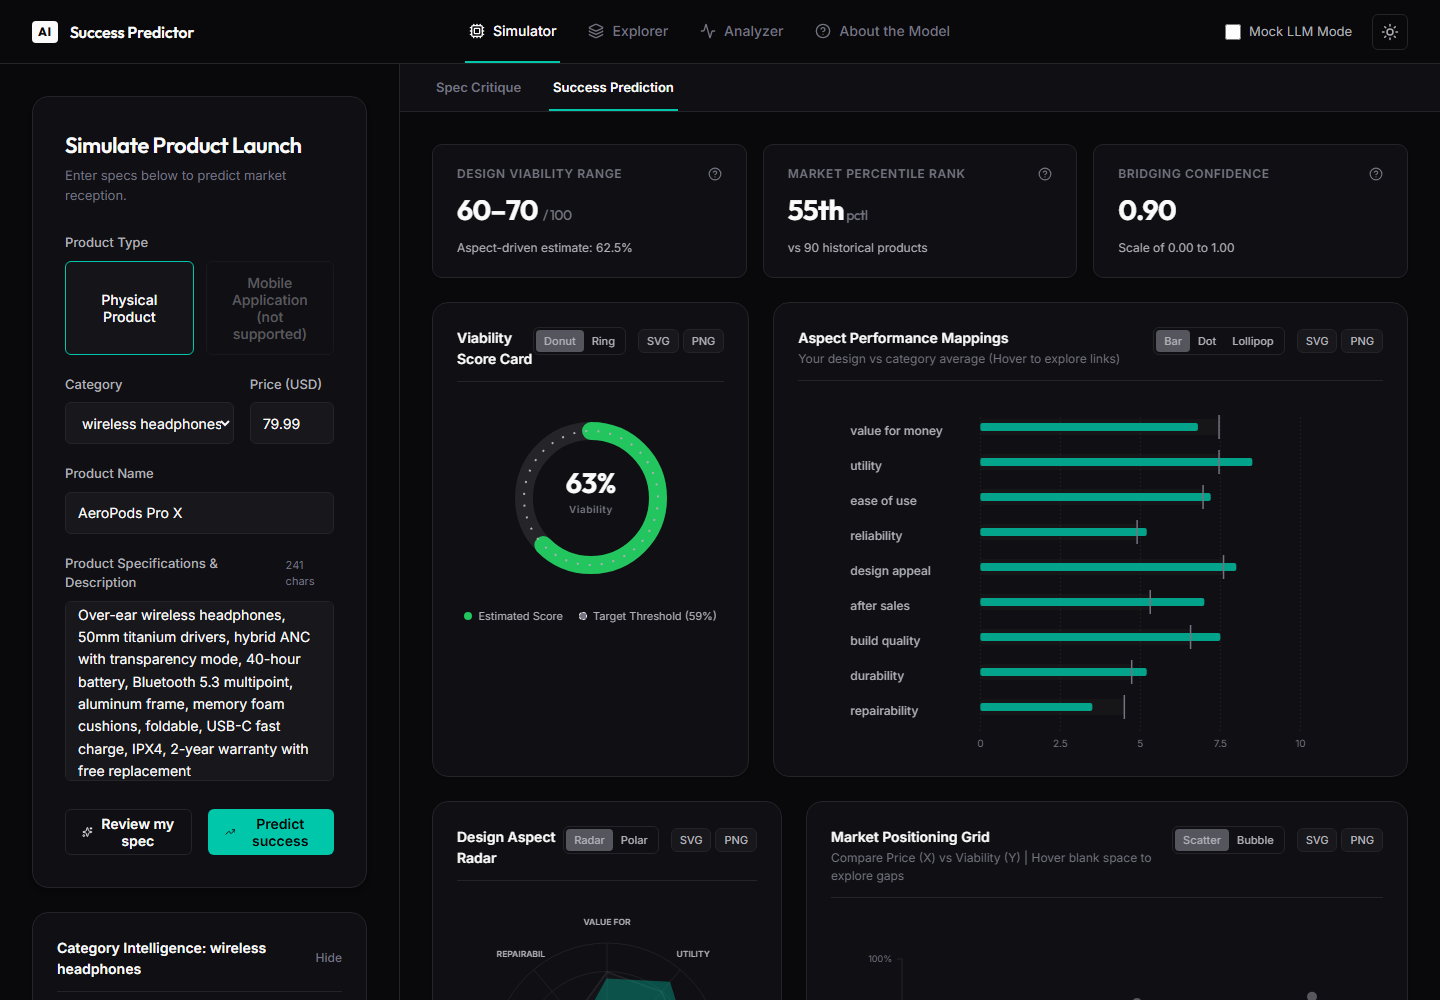
\includegraphics[width=\columnwidth]{fig6a_prediction.png}\\[2pt]
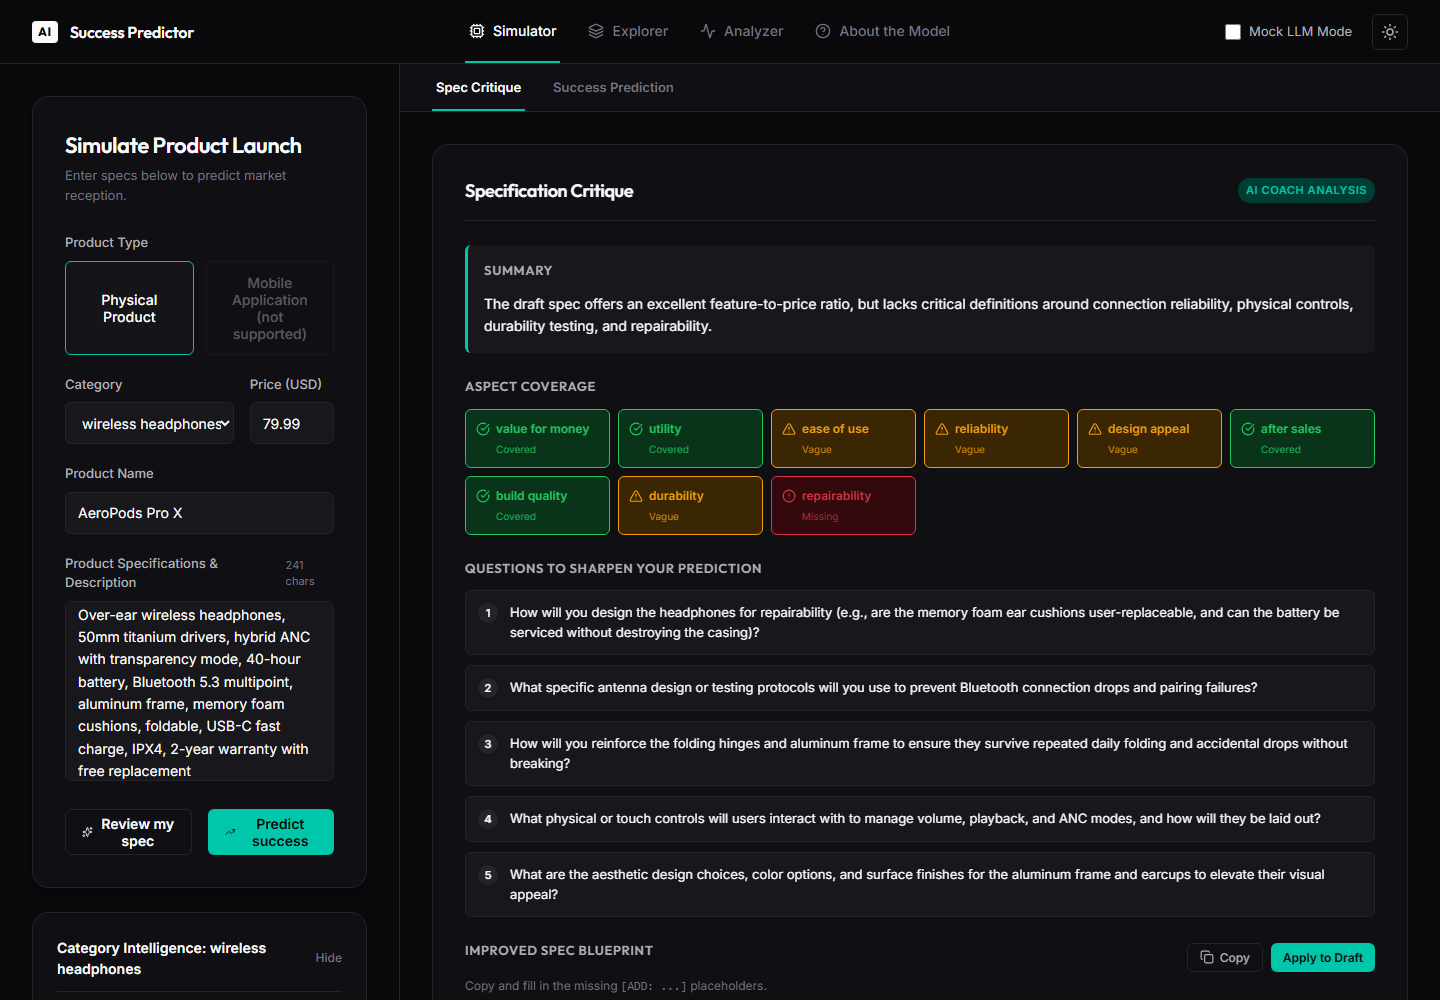
\includegraphics[width=0.49\columnwidth]{fig6b_spec_coach.png}\hfill
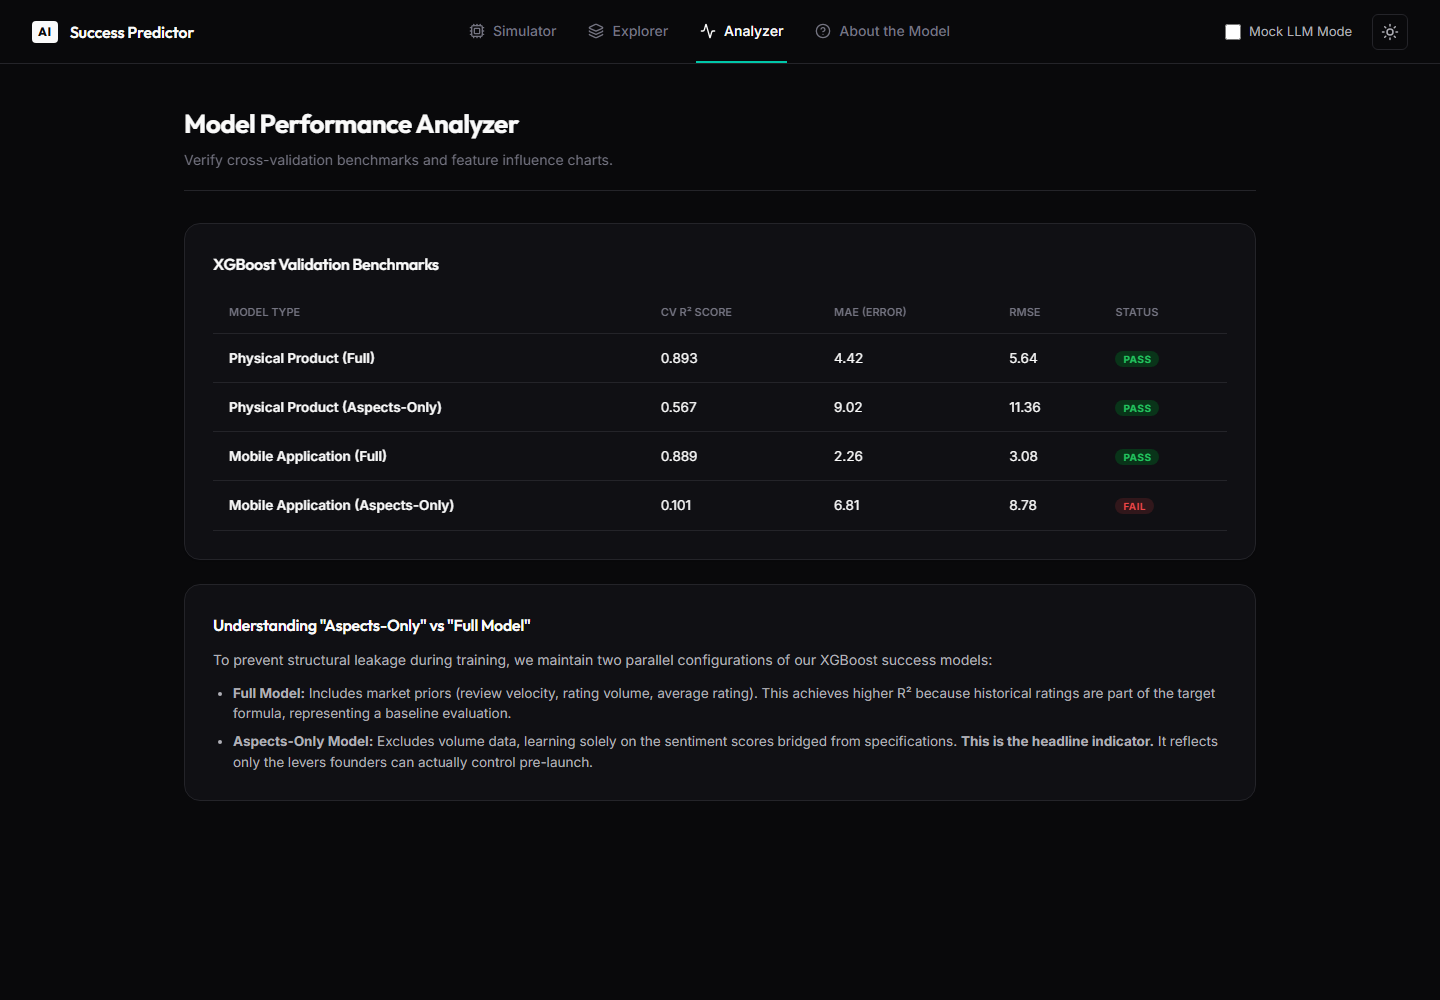
\includegraphics[width=0.49\columnwidth]{fig6c_analyzer.png}
\caption{The application. (a)~Prediction dashboard with viability range, percentile rank, aspect-vs-category chart, and the disabled app track. (b)~Spec coach. (c)~Analyzer view showing the honest benchmark table including the failed app-track gate.}
\label{fig:ui}
\end{figure}

\section{Limitations}
\label{sec:limitations}
\textbf{Survivorship bias is the most important limitation, and it bounds every claim in this paper.} The corpus requires at least five reviews per product, so products that launched and drew no attention, arguably the truest flops, are simply absent. Every result here is about ranking among products that reached the market's attention. Whether the system could flag a product destined to gain no traction at all is untested, and with this data it is untestable.

The second limit is statistical power. The holdout has $n = 59$; its CI is compatible with a weak-to-moderate true effect, and $\rho \approx 0.32$ explains roughly 10\% of the rank variance. The right use is screening many candidate designs, not settling a single launch decision. The third is scope: the validated claims cover six physical categories only, the app track failed all five outcome definitions we tried, and the Reddit lift is unconfirmed. The fourth concerns the inputs. Our ``specifications'' are launch-day marketing copy, the closest launch-knowable proxy we can recover after the fact, but not the same as the engineering specs a team holds before production, and optimistic in ways the skeptic prompt reduces without removing. The fifth is reproducibility: the pipeline depends on hosted LLMs, and while prompts and seeds are frozen, provider models change over time, so exact reproduction needs the archived extraction outputs we publish with the code. Last, review text can be gamed. The fraud filter removed 71 suspect products, but a sophisticated manipulation \cite{mayzlin2014promotional} would slip through it.

\section{Conclusion}
We asked whether a product's market fate can be read, at least in part, from its specification alone, before any consumer has touched it. Within carefully stated bounds, the answer is yes. An LLM that extracts aspect sentiment from 74{,}000 reviews, a gradient-boosted model that learns which aspect profiles succeed, and a skeptic-prompted bridging layer that estimates those profiles from specs together produce a launch-blind signal of $\rho = 0.317$ (CI $[0.06, 0.54]$) against real market outcomes. It was confirmed on a pre-registered holdout, it is almost orthogonal to price, and it rises monotonically across success tiers from flops to category leaders.

The most durable contribution, we think, is not that point estimate but the map around it: which aspects a specification can predict (ease of use, utility, build quality), which it cannot (after-sales service, aesthetics), and which markets the method works in at all (physical goods, where quality is rewarded) as against where it fails under every outcome we tested (app stores, where distribution dominates). For the small businesses that motivated this work, a map like that is the difference between an oracle they should not trust and an instrument they can: a pre-production screen that shifts the odds toward products their users find worth paying for. A tool that knows its own limits and shows them, through trust badges, abstention, and uncertainty ranges, is the only honest form such a tool can take at the current state of the art.

\bibliographystyle{IEEEtran}
\bibliography{refs}

\end{document}
